\documentclass[article,type=msc,colorback,accentcolor=tud7b]{tudthesis}

\usepackage{hyperref}
\usepackage[a-1b]{pdfx}
\usepackage[ngerman,english]{babel}
\usepackage{amsmath}
\usepackage{array}
\usepackage{enumitem}
\usepackage{listings}
\usepackage{floatrow}
\usepackage{multirow}
\usepackage{subfig}
% Table float box with bottom caption, box width adjusted to content
\newfloatcommand{capbtabbox}{table}[][\FBwidth]
\restylefloat{table}
\newcolumntype{C}[1]{>{\centering\let\newline\\\arraybackslash\hspace{0pt}}m{#1}}
\newcolumntype{R}[1]{>{\raggedleft\let\newline\\\arraybackslash\hspace{0pt}}m{#1}}

\usepackage[
    backend=biber, % biber ist das Standard-Backend für Biblatex. Für die Abwärtskompatibilität kann hier auch bibtex oder bibtex8 gewählt werden (siehe biblatex-Dokumentation)
    style=alphabetic, %numeric, authortitle, alphabetic etc.
    autocite=plain, % Stil, der mit \autocite verwendet wird
    sorting=nty, % Sortierung: nty = name title year, nyt = name year title u.a.
    sortcase=false,
    url=false,
    hyperref=auto,
    maxcitenames=2,
]{biblatex}

\addbibresource{bibliography.bib}

\newcommand{\getmydate}{%
  \ifcase\month%
    \or Januar\or Februar\or M\"arz%
    \or April\or Mai\or Juni\or Juli%
    \or August\or September\or Oktober%
    \or November\or Dezember%
  \fi\ \number\year%
}

\begin{document}
  \thesistitle{Sentiment Classification of Chess Annotations}{}
  \author{Florian Beck}
  \referee{Prof. Dr. Johannes Fürnkranz}{Dr. Markus Zopf}
  \department{Fachbereich Informatik}
  \group{Knowledge Engineering Group}
  \dateofexam{\today}{\today}
  \makethesistitle
  \selectlanguage{ngerman}
  \affidavit{Florian Beck}
  
  % INFO
% abstract.tex
% Für den Abstract der Abschlussarbeit oder Dissertation

\begin{abstract}
  Dies ist der Abstract der Arbeit.
  Er gibt wertungsfrei, kurz und prägnant den Inhalt der wissenschaftlichen Arbeit wieder.
\end{abstract}  


  \clearpage
  
  % INFO
% abstract.tex
% Für den Abstract der Abschlussarbeit oder Dissertation

\begin{abstract}
  Dies ist der Abstract der Arbeit.
  Er gibt wertungsfrei, kurz und prägnant den Inhalt der wissenschaftlichen Arbeit wieder.
\end{abstract}  


  \clearpage
  
  \selectlanguage{english}
  \setcounter{tocdepth}{6}
  \tableofcontents
  \setcounter{page}{6}
  \clearpage
  
  \listoffigures
  \listoftables
  \clearpage
  
  \section{Introduction}
    Chess games are noted in a uniform form like the PGN format in order to be able to perform analyses and evaluations at a later date. These data usually contain information about the players and the event as well as the exact move sequence of the chess game. In addition, especially in large chess databases, decisive moves and positions are provided with comments after the game has been analyzed by grandmasters. For a better arrangement of these comments there are standardized symbols and NAGs, which for example directly indicate whether a move was good or bad. These have the advantage that they are easier to evaluate due to their clear categorization and are also generally understandable, which is not the case with comments in natural language. \\\\
    In many cases the comments were therefore replaced by the annotation symbols if a comment did not seem necessary. For more detailed explanations, which can not only be expressed with an annotation symbol, both annotation symbols and comments are used. Finally, there are comments without a corresponding annotation symbol. This may be intentional if the commentary only names the commentator, summarizes a game or refers to similar chess games. However, some comments refer specifically to moves and positions and could therefore be provided with an annotation symbol. \\\\
    For the evaluation of annotation symbols in chess there are already approaches as described in \autocite{Wirth2014} and \autocite{Wirth2015}, where the annotations are used to learn preferences. In order to be able to use pure comment data for such evaluations, annotation symbols must have been assigned to the comments beforehand.

  \subsection{Problem Definition}
    In this thesis, a suitable approach for the correct assignment of annotation symbols to given chess annotations is to be found. It is a specialization of a supervised sentiment classification problem since the used data for the learning process contains only comments that are already labeled with the correct annotation symbol. This problem is split up into five separate questions:
    \begin{itemize}
      \item the correct categorization into move- and position-annotating comments for given chess comments
      \item the correct assignment of two annotation symbols $(!, ?)$ to given chess move comments
      \item the correct assignment of six annotation symbols $(!!, !, !?, ?!, ?, ??)$ to given chess move comments
      \item the correct assignment of three annotation symbols $(+-, =, -+)$ to given chess position comments
      \item the correct assignment of seven symbols $(+-, \pm, +=, =, =+, \mp, -+)$ to given chess position comments
    \end{itemize}

  \subsection{Goal of the Thesis}
    The main question of this work is whether and how well the appropriate annotation symbol for a given chess comment can be determined. Thus, the goal to find the configuration with the best accuracy and other evaluation metrics with regard to the classification problems just presented. For this purpose, four data models will be developed, ten classifiers selected and the configurations tested on three different data sets. In addition, further suitable processing methods are to be investigated and, if appropriate, added in order to optimize the results. The final analysis is also intended to provide insights into the remaining possibilities for improvement.
    
  \subsection{Structure of the Thesis}
    The thesis is split into five more chapters: \\\\
    The second chapter initially provides background knowledge in the topics dealt with in this thesis. It starts with the presentation of sentiment analysis as part of text mining. Afterwards the concept of word embeddings is discussed, which can serve as a data model in such text mining problems. This is followed by a description of multiclass classification problems and several suitable approaches to solve such problems. A separate look is taken at the subgroup of ordinal classification problems.  Finally, cost-sensitive methods are presented that take into account different weightings of misclassifications. \\\\
    The third chapter describes the general concept with which a text mining process can be created. It first deals with the requirements of problem and goal definition and the criteria for a suitable data selection. For the preparation of the data and their transformation into a model suitable for analysis, methods of natural language processing are presented. Finally, possible analysis methods and evaluation methods are presented from which suitable techniques for the problem can be selected. \\\\
    In the fourth chapter, the procedure presented in the third chapter is applied to the text mining process in chess annotations. First the format PGN and the annotation symbols NAG are explained and the five problems are specified. In the following the used tools like NLTK, Weka and further libraries are listed. Finally, the classifiers and evaluation methods used are mentioned. \\\\
    The fifth chapter contains all results and their evaluations. After the analysis of different tokenizer configurations, statistics about the comments are generated, which can be used to gain basic knowledge about the analyzed data set. In addition, the attributes and models used for the data set are evaluated. The majority of the results are finally taken up by the comparisons of the achieved accuracies for all configurations and problems. In the end, the best results achieved are checked for optimality in a cost-sensitive evaluation. \\\\
    The last chapter summarizes the most important conclusions from the results and gives an outlook which further approaches could be used to improve the results.
  \clearpage
  
  \section{Fundamentals}
    This chapter deals with some basics of the topics into which the problem discussed in the paper can be categorized. The first two sections Sentiment Analysis and Word Embeddings focus on data mining approaches for data in natural language. The remaining three sections Multiclass Classification, Ordinal Classification and Cost-sensitive Learning address the analysis and evaluation of data in (non-binary) classification problems.
  
  \subsection{Sentiment Analysis}
    Sentiment analysis, also known as sentiment classification or opinion mining, is the field of study that analyzes people’s opinions, sentiments, evaluations, attitudes and emotions from written language. It is one of the most active research areas in natural language processing and is also widely studied in data mining, Web mining, and text mining \autocite{Liu2012}. Due to the rapidly increasing amount of data on the Internet and the Web, the data sources for sentiment analysis have also grown considerably. In particular, since the spread of Web 2.0, more and more people have actively participated in the exchange of knowledge or opinions via the Internet. This results in large amounts of data of natural language, which are, however, often characterized by subjectivity. \\\\
    Nowadays, in addition to the large area of data in social media, evaluations of products and services play an important role in sentiment analysis. Between 73\% and 87\% of the consumer report that online product evaluations influence their purchase decision and with very good evaluations even a 20\% - 99\% higher price is accepted, whereby the exact added value depends on the product \autocite[section~1.1]{Pang2008}. Since these data are available in very large quantities, an automatic evaluation is desirable. \\\\
    Sentiment classification problems can occur at different levels of difficulty. \citeauthor{Plutchik1980} distinguishes in his model between the eight emotions joy, trust, fear, surprise, sadness, disgust, anger and anticipation. For each of these emotions there is a mild and an intense form, e.g. annoyance is the mild and rage the intense form of anger. The arrangement of similar emotions next to each other and opposing emotions opposite to each other results in Plutchik's wheel of emotions, which can be seen in figure~\ref{fig:plutchik_wheel} \autocite{Plutchik1980}.  
  
    \begin{figure}[H]
      \centering
      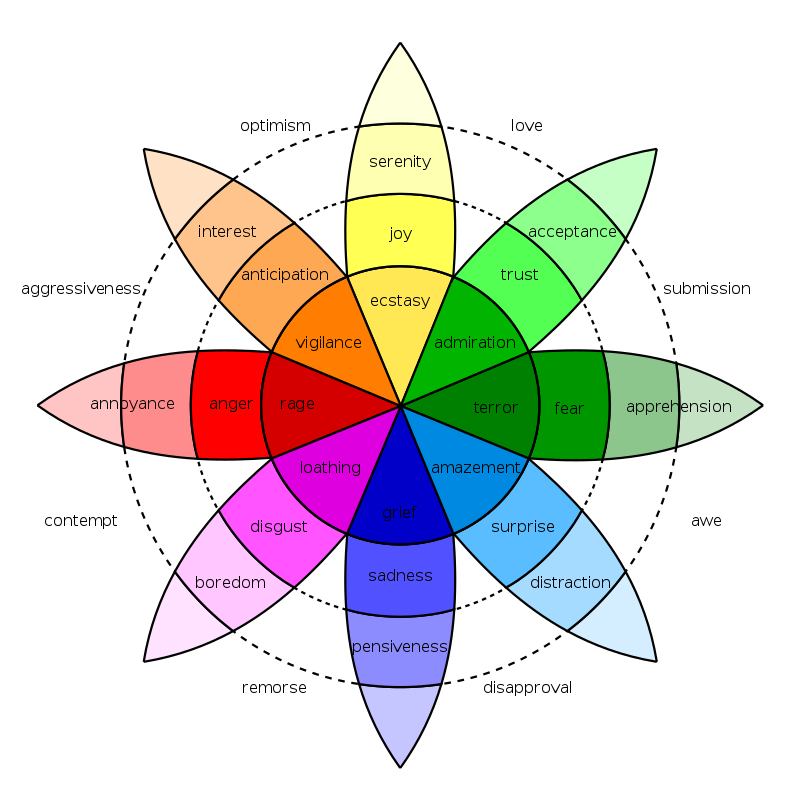
\includegraphics[scale=0.35]{images/plutchik_wheel}
      \caption[Plutchik's wheel of emotions]{Plutchik's wheel of emotions\protect\footnotemark}
      \label{fig:plutchik_wheel}
    \end{figure}
    
  	\footnotetext{\url{https://en.wikipedia.org/wiki/Robert_Plutchik\#/media/File:Plutchik-wheel.svg}, (07.05.2019, 06:24)}
  
    In most cases, however, a single scale is sufficient to classify the author's opinion. The only distinction is made between a positive and a negative attitude. With the help of sentiment words such as "good", "great" or "terrible" a reliable statement about the expressed opinion can be made quickly. These sentiment words are collected in various encyclopedias and are constantly being further developed. Nevertheless, some complications can occur here as well.  Negated sentences can contain sentiment words, but their meaning and thus also their sentiment is reversed by the negation. This is even more complicated with sarcastic statements, in which the sentiment is reversed, although there is no negation in the text. Finally, there are also sentences that do not contain a single sentiment word and nevertheless express a clear opinion. An example of this is the sentence "This washer uses a lot of water", which implicitly expresses a negative attitude \autocite[section 1.2.2]{Liu2012}.  

  \subsection{Word Embeddings}
  \label{subsec:word_embeddings}
    The application of text mining or sentiment analysis strategies requires a suitable application of the documents to be analyzed, usually by converting them into machine-understandable numeric values. A common representation form of document in natural language processing is the vector space model. Each word which appears in at least one document, i.e. which is part of the vocabulary, forms a dimension in the vector space model. Finally, each document is represented as a vector in this vector space by assigning a number to each word in the vocabulary, e.g. its absolute or relative term frequency. This allows finding documents that contain certain words and comparing documents on the basis of their contained words using a distance function in the vector space. \\\\
    However, the vector space model has some limitations and disadvantages. These include the usually high number of dimensions caused by a big vocabulary, which results in high memory and computing costs. Moreover, it leads to sparse data, because most words of the vocabulary do not occur in a document and its value is therefore $0$. Besides, synonyms or similar words are treated in different dimensions and thus documents using those different words cannot be detected as similar. \\\\
    Word embeddings are a collection of techniques to map documents or single words to a vector space whereby the above-mentioned problems are solved. A predefined vector space of a fixed size $N$ is used and the approach of a distributed representation provides better and multiple degrees of similarities between two words. \citeauthor{Mikolov2013} developed a new word embedding model that not only reduces the count of dimensions heavily, but also offers large improvements in accuracy of semantic and syntactic questions \autocite{Mikolov2013}. Hence algebraic functions can be used to answer questions like the currency of a country: vector(“Euro”) $-$ vector(“Germany”) $+$ vector(“South Africa”) calculates a vector close to the vector(“Rand”). \\\\
    The underlying concept is based on a neural network with an input layer, an output layer and a hidden projection layer in between. \citeauthor{Mikolov2013} uses two different models shown in figure~\ref{fig:word_embeddings} that are both based on the context of the word. The continuous bag-of-words (CBOW) model gets the context of a word as the input, i.e. the $k$ preceding and $k$ succeeding words, in the figure with the so-called window size $k=2$. With the skip-gram model the input and output are reversed; from a given word, the context is inferred. In both cases, the output is a learned vocabulary, with a vector of the previously defined length $N$ assigned to each word \autocite{Mikolov2013}. Based on this vector, now further learning methods can be applied.
 
    \begin{figure}[H]
      \centering
      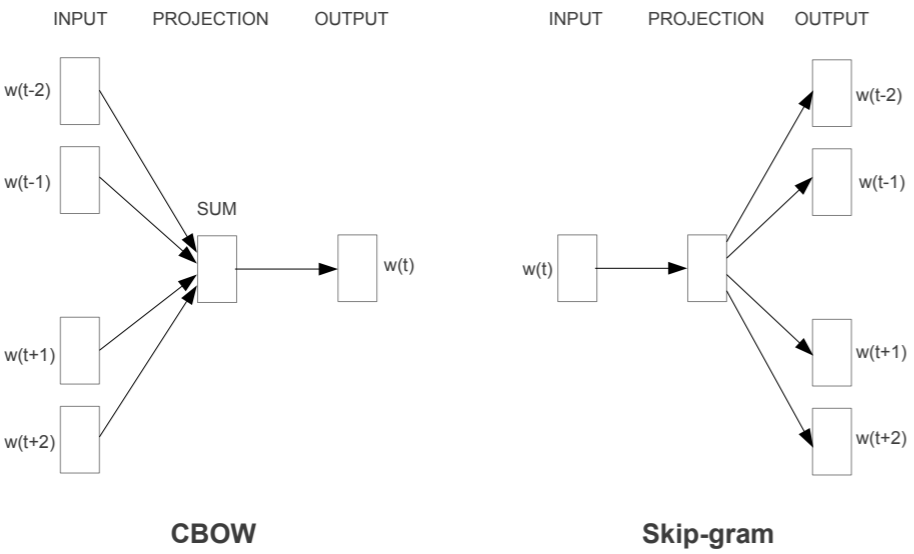
\includegraphics[scale=0.75]{images/word_embeddings}
      \caption[CBOW and Skip-gram model]{CBOW and Skip-gram model \autocite{Mikolov2013}}
      \label{fig:word_embeddings}
    \end{figure}
    
    Even if the output itself is compared to the traditional vector space model meaningless to a human, the combination of multiple vectors offers considerable information. In addition to the already mentioned use of algebraic functions, the vocabulary can be searched for synonyms or other related words by looking for a similar vector like the given word has. To calculate the similarity of two vectors, the cosine similarity can be used. Its value is between $-1$ indicating completely different words and $1$ indicating identical words, where $0$ stands for no correlation between the words. The cosine similarity of two vectors $\mathbf{a}$ and $\mathbf{b}$ is defined as follows:
    \[\cos (\theta)=\frac{\mathbf{a} \cdot \mathbf{b}}{\|\mathbf{a}\|_{2}\|\mathbf{b}\|_{2}}=\frac{\sum_{i=1}^{n} a_{i} \cdot b_{i}}{\sqrt{\sum_{i=1}^{n}\left(a_{i}\right)^{2}} \cdot \sqrt{\sum_{i=1}^{n}\left(b_{i}\right)^{2}}}\]
    \citeauthor{Kusner2015} compare several further measurements of similarity of words or documents and their performance in different corpora. They also present the Word Mover’s Distance (WMD), a novel distance function between text documents leading to unprecedented low $k$-nearest neighbor document classification error rates \autocite{Kusner2015}. \\\\
    The models presented by \citeauthor{Mikolov2013} as well as the cosine similarity measurements are implemented and collected in the framework word2vec and can be used for training and evaluation in the most common programming languages. Another common model is GloVe\footnote{\url{https://nlp.stanford.edu/projects/glove/}}, coined from Global Vectors, which in addition to the local context-based learning used in Word2Vec integrates global statistics of matrix factorization. The GloVe model produces a vector space with meaningful substructure, as evidenced by its performance of 75\% on a recent word analogy task \autocite{Pennington2014}. Both frameworks offer pre-learned word embeddings on big corpora, among them also topic-specific data sets. However, it is also possible to learn a new embedding on an own data set.
  
  \subsection{Multiclass Classification}
  \label{subsec:multiclass_classification}  
    Multiclass classification is a problem in the field of supervised learning. The task is the prediction of one class out of a finite set of three or more possible classes for each instance. As can be seen in figure~\ref{fig:problem_hierarchy_supervised_learning}, it can be distinguished from other problems in supervised learning. First, as the name implies, it is a classification problem because the range of values is finite rather than continuous, as is the case with a regression problem. Furthermore, each instance should be associated with exactly one class, which distinguishes it from the similar sounding multi-label classification, since each instance can be associated with any number of classes, also known as labels. Finally, the model to be learned has to choose from a set of $k$ classes with $k>2$, i.e. from a set $\{1,2,\dots,k\}$. This makes the problem slightly more difficult than binary classification with $k=2$. Ordinal classification is a specialization of multiclass classification and will be discussed in detail in section~\ref{subsec:ordinal_classification}.
    
    \begin{figure}[H]
      \centering
      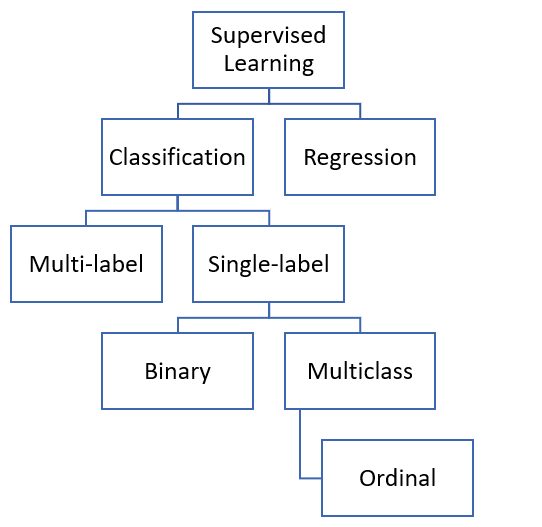
\includegraphics{images/problem_hierarchy_supervised_learning}
      \caption{Problem hierarchy of supervised learning}
      \label{fig:problem_hierarchy_supervised_learning}
    \end{figure}
    
    Most algorithms applied to classification problems are explained by their application to binary classification problems, which cover a large part of the real-world use cases. However, these approaches cannot be adopted to multiclass problems without further ado. \citeauthor{Aly2005} describes with the decomposition into binary classification, hierarchical classification and the extension of algorithms the three groups of approaches to cope with the difficulties of multiclass classification \autocite{Aly2005}:
    \begin{itemize}
      \item Decomposition into Binary Classification

        A frequently chosen approach is the transformation of the multiclass classification problem into several binary classification subproblems, for which there are three different possibilities. In any case the results of subproblems have to be joined to be able to make a final prediction which is similar to ensemble learning. \\\\
        The first option called one-against-all splits the multiclass classification problem into $k$ binary classification subproblems. The classifier $f_{i}$ treats the instances of class $i$ as positive and instances of the $k-1$ other classes as negative. An example of one-against-all using an SVM-classifier is shown in figure~\ref{fig:one_against_all}. For an unseen instance $x$ the class $k$ with the highest confidence score will be predicted:
        \[y(x)=\underset{i\in\{1 \dots k\}}{\operatorname{argmax}} f_{i}(x)\]
        However, there is no guarantee that the real-valued quantities $f_{i}(x)$ for different classifiers will have appropriate scales. Furthermore, especially for a high $k$ the ratio between positive and negative instances is low, which complicates the creation of a model. This problem can be addressed by giving greater weight to the positive instances \autocite[section~7.1.3]{Bishop2006}.

        \begin{figure}[H]
          \subfloat[One-against-all]{
            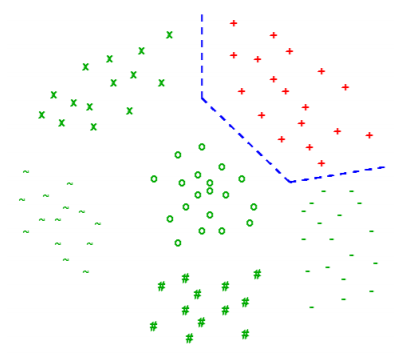
\includegraphics{images/one_against_all}
            \label{fig:one_against_all}
          }
          \quad
          \subfloat[One-against-one]{
            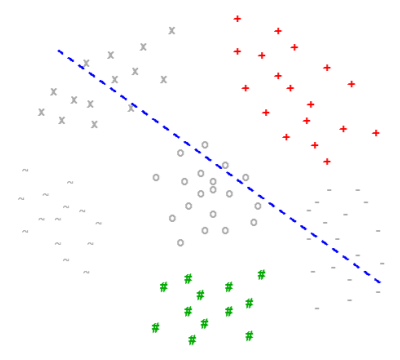
\includegraphics{images/one_against_one}
            \label{fig:one_against_one}
          }
          \caption[One-against-all vs. one-against-one approach]{One-against-all vs. one-against-one approach\protect\footnotemark}
        \end{figure}
    
        \footnotetext{J. Fürnkranz, Machine Learning and Data Mining | Learning Rule Sets, V3.0, p.45\&47}

        The second option called one-against-one splits the multiclass classification problem into even more binary classification subproblems, in fact $k(k-1)/2$. This number results from the fact that now in each subproblem two classes are pairwise distinguished from each other. Since in the binary classifier between the classes $i$ and $j$ all instances of the classes except $i$ and $j$ can be discarded (see figure~\ref{fig:one_against_one}), there are smaller subproblems than in one-against-all, which usually also create simpler models. However, the number of subproblems is $\frac{k}{2}$-times as high, which usually results in significantly more training time \autocite[section~7.1.3]{Bishop2006}. \\
        The final decision is made by voting. All pairwise comparisons are summed up and the winner with the most partial victories is the output class. However, using the binary outputs of the subproblems, i.e. only the preferred class, often leads to several winners. There are different ways to handle these ambiguities. The first idea is weighting the subproblems differently, for example by modifying the output from $1$ to the accuracy and from $0$ to $1-$accuracy. Another idea called pairwise coupling, which includes probabilities for every subproblem in the calculation, can be used to extend the one-against-one approach. \citeauthor{Wu2004} present a few pairwise coupling techniques that are more stable than using the simple voting approach \autocite{Wu2004}. \\\\

        The third option is the usage of error-correcting output codes. Each class is assigned to a unique binary string of length $n$; we will refer to these strings as “codewords”. During training for an example from class $i$, the desired outputs of these $n$ binary functions are specified by the codeword for class $i$. With artificial neural networks, these $n$ functions can be implemented by the $n$ output units of a single network \autocite[chapter~1]{Dietterich1994}. Though, it is also possible to train all $n$ binary classifiers individually with an arbitrary algorithm. A test instance is assigned to the class that is closest to the code determined by the $n$ functions. \\
        Now the question arises, how the codewords respectively the binary functions are chosen most effectively. Out of all $2^{k}$ binary combinations for a $k$-class problem, after removing $2^{k-1}$ complements (e.g. all starting with $1$) and the uniform classifier there are $2^{k-1}-1$ possible classifiers, from which to be selected. A good error-correcting output code for a $k$-class problem should satisfy two properties \autocite[section~2.3]{Dietterich1994}:
        \begin{itemize}
          \item Row Separation

            If in a code converting an arbitrary codeword into another arbitrary codeword needs $d$ changes of bits, the code has a so-called Hamming distance of $d$. The higher the Hamming distance, the better the row separation. A code with Hamming distance $d$ can detect up to $d-1$ and correct up to $\left\lfloor\frac{d-1}{2}\right\rfloor$ bits.
          \item Column Separation

            Each bit-position function $f_{i}$ should be uncorrelated with the functions to be learned for the other bit positions $f_{j}$; $j\neq i$. If two columns $i$ and $j$ (or the complement of $j$) are similar or identical, then when a deterministic learning algorithm such as the decision tree classifier C4.5 is applied to learn $f_{i}$ and $f_{j}$, it will make similar (correlated) mistakes.
        \end{itemize}
        The classifier sets in the one-against-all and one-against-one approaches are feasible solutions. The one-against-all approach guarantees Hamming distances of $2$ for both row and column separation, the one-against-one approach even $2\times(k-2)$ for the row and $4$ (if $k>7$) for the column separation. The optimal row distance is achieved by the union of all $2^{k-1}-1$ binary combinations and called exhaustive code. Until $k=5$ the exhaustive code is just the union of all classifiers of the one-against-all and one-against-one approaches (or their inversions, see table~\ref{tab:exhaustive_ecoc}), but for $k>6$ the number of additional classifiers increases quickly, wherefore instead of an exhaustive code also a suitable subset of those classifiers can be sufficient and improve the column separation.
  
        \begin{table}[H]
          \centering
          \setlength\tabcolsep{1.5pt}
          \subfloat[One-against-all]{
          \begin{tabular}{ |C{1.5cm}|C{0.5cm}|C{0.5cm}|C{0.5cm}|C{0.5cm}|C{0.5cm}| } 
            \hline
            class & $f_{1}$ & $f_{2}$ & $f_{3}$ & $f_{4}$ & $f_{5}$ \\ \hline
            1 & 1 & 0 & 0 & 0 & 0 \\ \hline
            2 & 0 & 1 & 0 & 0 & 0 \\ \hline
            3 & 0 & 0 & 1 & 0 & 0 \\ \hline
            4 & 0 & 0 & 0 & 1 & 0 \\ \hline
            5 & 0 & 0 & 0 & 0 & 1 \\ \hline
          \end{tabular}
          }
          \quad
          \subfloat[One-against-one]{
          \begin{tabular}{ |C{1.5cm}|C{0.5cm}|C{0.5cm}|C{0.5cm}|C{0.5cm}|C{0.5cm}|C{0.5cm}|C{0.5cm}|C{0.5cm}|C{0.5cm}|C{0.5cm}| } 
            \hline
            class & $f_{1}$ & $f_{2}$ & $f_{3}$ & $f_{4}$ & $f_{5}$ & $f_{6}$ & $f_{7}$ & $f_{8}$ & $f_{9}$ & $f_{10}$ \\ \hline
            1 & 1 & 1 & 1 & 1 & 0 & 0 & 0 & 0 & 0 & 0 \\ \hline
            2 & 1 & 0 & 0 & 0 & 1 & 1 & 1 & 0 & 0 & 0 \\ \hline
            3 & 0 & 1 & 0 & 0 & 1 & 0 & 0 & 1 & 1 & 0 \\ \hline
            4 & 0 & 0 & 1 & 0 & 0 & 1 & 0 & 1 & 0 & 1 \\ \hline
            5 & 0 & 0 & 0 & 1 & 0 & 0 & 1 & 0 & 1 & 1 \\ \hline
          \end{tabular}
          }
      
          \subfloat[Exhaustive error-correcting output code]{
          \begin{tabular}{ |C{1.5cm}|C{0.5cm}|C{0.5cm}|C{0.5cm}|C{0.5cm}|C{0.5cm}|C{0.5cm}|C{0.5cm}|C{0.5cm}|C{0.5cm}|C{0.5cm}|C{0.5cm}|C{0.5cm}|C{0.5cm}|C{0.5cm}|C{0.5cm}| } 
            \hline
            class & $f_{1}$ & $f_{2}$ & $f_{3}$ & $f_{4}$ & $f_{5}$ & $f_{6}$ & $f_{7}$ & $f_{8}$ & $f_{9}$ & $f_{10}$ & $f_{11}$ & $f_{12}$ & $f_{13}$ & $f_{14}$ & $f_{15}$ \\ \hline
            1 & 0 & 0 & 0 & 0 & 0 & 0 & 0 & 0 & 0 & 0 & 0 & 0 & 0 & 0 & 0 \\ \hline
            2 & 0 & 0 & 0 & 0 & 0 & 0 & 0 & 1 & 1 & 1 & 1 & 1 & 1 & 1 & 1 \\ \hline
            3 & 0 & 0 & 0 & 1 & 1 & 1 & 1 & 0 & 0 & 0 & 0 & 1 & 1 & 1 & 1 \\ \hline
            4 & 0 & 1 & 1 & 0 & 0 & 1 & 1 & 0 & 0 & 1 & 1 & 0 & 0 & 1 & 1 \\ \hline
            5 & 1 & 0 & 1 & 0 & 1 & 0 & 1 & 0 & 1 & 0 & 1 & 0 & 1 & 0 & 1 \\ \hline
          \end{tabular}
          }
          \caption[Output codes for a multiclass classification problem]{Different output codes for a multiclass classification problem with five classes}
          \label{tab:exhaustive_ecoc}
        \end{table}

        The exhaustive error-correcting code for $k=5$ is shown in table~\ref{tab:exhaustive_ecoc}. The hamming-distance of the code is $d=8$. Therefore, the code can detect up to $d-1=7$ and correct up to $\left\lfloor\frac{d-1}{2}\right\rfloor=3$ bits. Error-correcting output codes are a robust alternative to one-against-all and one-against-one approaches which outperforms them in most cases but also entail the disadvantages of a more complex training and model \autocite[chapter~4]{Dietterich1994}.
      \item Hierarchical Classification

        Hierarchical classification, also known as nested dichotomies, is strictly speaking also a type of decomposition of a multiclass classification problem into binary classification problems. However, in this approach the output of the classifiers is not always used for the prediction but as the input for the next classifier. In this way, a hierarchy of classifiers and their subproblems is created. The first classifier is trained on the whole input space; the total set of all classes is suitably divided into two subsets between which the classifier distinguishes. This procedure is then continued recursively with the two subsets until all subsets only contain instances of a single class. This procedure creates a tree structure whose leaves are the set of instances of a class. As a result, this tree contains $k$ leaves and $k-1$ inner nodes representing the binary classifiers \autocite{Dong2005}. Two possibly outcomes of a multiclass classification problem with $5$ classes are shown in figure~\ref{fig:nested_dichotomies}.

        \begin{figure}[H]
          \centering
          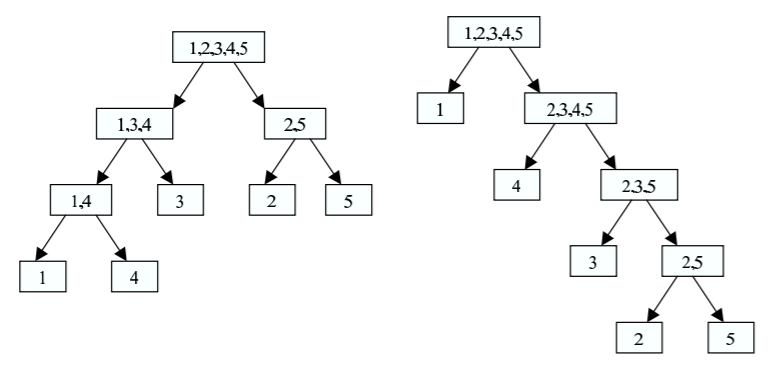
\includegraphics{images/nested_dichotomies}
          \caption[Two nested dichotomies]{Two nested dichotomies for a multiclass problem with five classes \autocite{Dong2005}}
          \label{fig:nested_dichotomies}
        \end{figure}

        The probability of a class can be calculated by multiplying all probability estimates of the classifier along the path from the root to the class. This value differs for disparate nested dichotomies, wherefore usually various trees are computed and their probabilities are averaged. Though, for high $k$ there are too many different possibilities to build a nested dichotomy. Balanced nested dichotomies prove to be particularly suitable, since they require the shortest running time without affecting the accuracy negatively \autocite{Dong2005}. \citeauthor{Dong2005} developed methods to balance the nested dichotomies either by class or by data amount, i.e. the subsets are created in a way that either their difference of classes or their difference of data is minimal. The left dichotomy shown in figure~\ref{fig:nested_dichotomies} is class-balanced, because the difference of classes between all subsets is either zero or one. It is as well data-balanced, if all classes have nearly the same number of instances. The right dichotomy is not class-balanced, because the first two splits have class ratios of $4:1$ and $3:1$. However, this dichotomy is data-balanced if class $1$ contains nearly as much instances as all other classes, class $2$ nearly as much as $3$, $4$ and $5$ together and class $3$ as much as $4$ and $5$ together.
      \item Extension of Algorithms

        The third idea is the inversion of the first two approaches. Instead of modifying the problem and using the same classifier as for the binary classification, we now modify the classifier such that we can leave the classifier unchanged. Typical algorithms in machine learning are decision trees, pattern- or rule-based classifiers, probabilistic classifiers, SVM classifiers, neural network classifiers and proximity-based classifiers. A short description for every algorithm can be found in section~\ref{subsec:analysis}. Decision trees, pattern- or rule-based classifiers, probabilistic classifiers as Naïve Bayes and proximity-based classifiers as $k$-nearest-neighbor can be easily adapted to multiclass problems. For the other two algorithms some preliminary considerations are necessary. \\\\
        SVM classifiers use hyperplanes of dimension $D-1$ described by linear functions to separate the whole input space of dimension $D$ into two subspaces which ideally only contain a single class. Obviously, a single hyperplane is not sufficient for separating more than two classes. Approaches like one-against-all and one-against-one lead to ambiguous subspaces where either more than one class or no class is assigned to. We can avoid these difficulties by considering a single $k$-class discriminant comprising $k$ linear functions (with parameters $\mathbf{w}_{i}$ and $w_{i 0}$) of the form
        \[y_{i}(\mathbf{x})=\mathbf{w}_{i}^{\mathrm{T}} \mathbf{x}+w_{i 0}\]
        and then assigning a point $\mathbf{x}$ to class $i$ if $y_{i}(\mathbf{x})>y_{j}(\mathbf{x})$ for all $j\neq i$. The decision boundary between class $i$ and class $j$ is therefore given by $y_{i}(\mathbf{x})=y_{j}(\mathbf{x})$ and hence corresponds to a $(D-1)$-dimensional hyperplane defined by
        \[\left(\mathbf{w}_{i}-\mathbf{w}_{j}\right)^{\mathrm{T}} \mathbf{x}+\left(w_{i 0}-w_{j 0}\right)=0.\]
        The decision regions of such a discriminant are always singly connected and convex \autocite[section~4.1.2]{Bishop2006}. \\\\
        A neural network classifier has in general $n$ neurons in the output layer, each of them with a binary output. For binary classification problems, a single neuron in the output layer, i.e. $n=1$, is sufficient since it only needs to distinguish between two classes, represented by the two outputs $0$ and $1$. For multiclass classification problems, $n=1$ is not sufficient. The straightforward solution would be to define $n=k$ neurons in the output layer, one for each of the $k$ classes. But already $\left\lfloor\log_{2}k\right\rfloor$ output neurons are enough if the classes are encoded as the first $k$ numbers in binary representation. By using error-correcting output codes containing more than $\left\lfloor\log_{2}k\right\rfloor$ output neurons, the binary code can also be made more resistant to errors \autocite[section~2.1]{Aly2005}.
    \end{itemize}
    As mentioned in the beginning of this section, ordinal classification problems are a subgroup of multiclass classification problems. The following section describes the special properties of this type of problems and other approaches that are even better adapted to these properties than those presented here.

  \subsection{Ordinal Classification}
  \label{subsec:ordinal_classification}
    Ordinal classification problems are a specialization of multiclass classification problems. They refer to an important category of real-world problems, in which the classes exhibit a natural order. Thus, the class attribute is not nominal, but ordinal. However, the possibility of calculating the difference (essential for an interval class attribute) or even the quotient (essential for a ratio class attribute) is usually not given \autocite[chapter~1]{Frank2001}. Ordinal classification may be viewed as a bridging problem between the two standard machine-learning tasks of classification and regression, because the set of classes has the property of a finite range given in classification problems as well as the property of a natural order given in regression problems \autocite[chapter~1]{Kotsiantis2004}. \\\\
    As a specialization of a multiclass classification problem, ordinal classification problems can be approached with the same strategies as described above in section~\ref{subsec:multiclass_classification}. However, the additional information of the linear order of the classes is ignored. Two strategies tailored to ordinal classification problems taking this information into account are ordinal regression and an adapted transformation to binary classification problems.
    \begin{itemize}
      \item Ordinal Regression

        In regression tasks, the output is a numeric value in a continuous range. The idea of ordinal regression is to treat the ordinal output as a numeric value. In this way the same approaches as for regression tasks can be used only with the extension that the predicted values still have to be mapped to the fixed classes. Nevertheless, most regression methods require some metric assumptions like building differences or ratios within the ordinal scale \autocite[chapter~1]{Ruan2014}. Hence the result of the model depends on the choice of numeric values and their distances from each other. This leads to problems in many real-world applications, for example in the quantification of ordinal scales in opinion surveys. \\\\
        Ordinal logistic models avoid this issue by only considering the ranking order of the classes \autocite[chapter~13]{Harrell2015}. The most commonly used ordinal logistic model is the proportional odds model. It uses the logarithms of odds that the predicted class $y$ is one of the first $i$ classes together with a linear function, whereby the probability after forming is given by
        \[\operatorname{P}(y\leq i|\mathbf{x})=\frac{1}{1+\exp\left[-\left(\mathbf{w}^{\mathrm{T}}\mathbf{x}+w_{i 0}\right)\right]}\]
        where $\mathbf{x}$ is the test instance and $\mathbf{w}$ and $w_{i 0}$ the parameters of the linear function. There are many possible extensions to this ordinal model, among others replacing the cumulative probabilities with conditional probabilities or using a hazards model \autocite[chapter~13]{Harrell2015}. 
      \item Transformation to Binary Classification Problems
      
        A simpler approach using a transformation to binary classification problems is presented by \citeauthor{Frank2001}. In contrast to the binary classification approaches in multiclass classification it takes advantage of the order of the classes. The ordinal class attribute with ordered values $v_{1}<v_{2}<\ldots< v_{k}$ is converted into $k-1$ binary attributes. The $i$-th binary attribute represents the test if the class attribute $y$ exceeds the value of the $i$-th class: $y>v_{i}$. This construction of binary attributes requires exactly two classifiers and their probabilities to determine whether a test instance $\mathbf{x}$ belongs to a class $i$:
        \[\operatorname{P}\left(y=v_{i}\mid\mathbf{x}\right)=\operatorname{P}\left(y>v_{i-1}\mid\mathbf{x}\right)-\operatorname{P}\left(y>v_{i}\mid\mathbf{x}\right)\]
        For the lowest class, the first probability is $1$ and for the highest, the second is $0$, which further simplifies the calculation. Finally, the class with the highest probability is predicted. \citeauthor{Frank2001} showed that for ordinal classification problems this approach outperforms the “naïve” one-against-all algorithm, which treats the class values as an unordered set \autocite{Frank2001}.
    \end{itemize}
  
  \subsection{Cost-sensitive Learning}
  \label{subsec:cost_sensitive_learning}
    In many classification problems the goal is the optimization of some performance measurement, most often the accuracy. However, the best solution in respect to the accuracy does not have to be the one with minimized costs, which is also often a goal to be achieved. Costs cannot only arise from misclassifications, but also from additional tests or time for the creation of a better model. \citeauthor{Turney2002} divides the reasons for costs that a machine learning problem can entail into nine groups \autocite{Turney2002}:
    \begin{itemize}[noitemsep]
      \item misclassification errors
      \item tests
      \item teacher
      \item intervention
      \item unwanted achievements
      \item computation
      \item cases
      \item human-computer interaction
      \item instability
    \end{itemize}
    In each of the nine groups, a distinction can be made between constant and conditional costs. In the case of test costs, we speak of constant costs if a certain test has a fixed cost value for its execution. Note that different test may have different costs if they still remain constant for all instances in all circumstances. On the contrary, conditional test costs depend on a criterion. For a medical test this criterion might be the test result, the age of a patient or the result of prior tests. In the remaining section, of all cost types only the misclassification costs are discussed and therefore abbreviated to costs. \\\\
    The standard approach to evaluate the performance of a classifier is the calculation of the accuracy, i.e. the number of correct classified instances in relation to the total number of instances. The error costs result directly from the number of misclassified instances, which only has to be multiplied by a constant cost factor. Thus, \citeauthor{Turney2002} calls this value constant misclassification error cost. However, there are various problems in machine learning where such a simplification would lead to a miscalculation of the total costs because the conditional error costs are ignored. \\\\
    In many cases, the equal treatment of all error types is the cause of the incorrect cost estimate. For this we first consider the binary classification with only two classes and therefore only two possible error types. A false positive (FP) occurs when the outcome is incorrectly predicted as yes or positive when it is actually no or negative. The reverse case is called false negative (FN). False positives and false negatives have rarely equal costs in real-world applications. In spam-classification, a no-spam e-mail classified as spam is worse than a spam e-mail which have not been detected correctly. An accepted customer which is not capable of paying back a loan has bigger costs than a customer wrongly classified as insolvent. A sick patient who is classified as healthy is more problematic than a healthy patient who is classified as sick. In order to map this, a cost value is determined for each of the two errors FP and FN or the cost ratio is determined. \\\\
    If we transfer the cost calculation to the multiclass classification, there are more error types and therefore more cost factors to be defined: Each instance of class $i$, misclassified as class $j$ will be multiplied with the correspondent cost factor $c_{ij}$. For a multiclass classification problem with $n$ classes we get a $n\times n$ cost matrix similar to the confusion matrix, which has $n(n-1)$ possibly different cost factors and whose main diagonal contains zeros. \\\\
    A special case arises for classification problems with ordinal classes. The value of $c_{ij}$ should reflect the extent of the difference between $i$ and $j$. Thus, it is common to assume that $c_{ij}=0$ when $i=j$. In addition, the cost $c_{ij}$ is assumed to be larger when $i$ is further away from $j$. Two common functions satisfy the requirements and have been widely used in practice \autocite[section~3.1]{Ruan2014}:
    \begin{itemize}
      \item \makebox[4cm][l]{Absolute cost vectors} $c_{ij}=\left|i-j\right|$
      \item \makebox[4cm][l]{Squared cost vectors} $c_{ij}=\left(i-j\right)^{2}$
    \end{itemize}
    Note that the squared cost charges more than the absolute cost when $i$ is further away from $j$ since $\left|i-j\right|\geq1\forall i,j\in\mathbb{Z}$. The cost matrix of a multiclass classification problem with $n$ classes using absolute cost vectors looks like this \autocite[chapter~3]{Kotsiantis2004}:
    \[\left[ \begin{array}{ccccc}
    {0} & {1} & {2} & {\dots} & {n-1} \\
    {1} & {0} & {1} & {\dots} & {n-2} \\
    {\dots} & {\dots} & {\dots} & {\dots} & {\dots} \\
    {n-2} & {\dots} & {1} & {0} & {1} \\
    {n-1} & {\dots} & {2} & {1} & {0}
    \end{array}\right]\]
    By squaring each element of the matrix, one obtains the matrix of squared cost vectors. In both cases it is a symmetrical matrix, i.e. $c_{ij}=c_{ji}\forall i,j\in\{1, \dots, m\}$. In some cases, it may be useful to weight the over- and underestimation of classes differently. If the overestimation of a class is to be penalized more severely than the underestimation, all elements to the right of the main diagonal are multiplied by a constant value $\lambda>1,\lambda\in\mathbb{R}$. In a comparable way all values of the matrix can be adjusted as required to the problem which has to be solved. \\\\
    Given such a cost matrix, the cost of a particular learned model on a given test set can be calculated just by summing the relevant elements of the cost matrix for the model’s prediction for each test instance. Here, the costs are ignored when making predictions, but taken into account when evaluating them \autocite[section~5.7]{Witten2005}. In this way the classifier obviously does not have to deliver the cost-optimal result. However, there are different possibilities to include costs in advance \autocite[section~2.3]{Qin2010}:
    \begin{itemize}
      \item Change of the class distribution of the training data
        
        This approach incorporates the misclassification cost into the data pre-processing step by re-sampling or re-weighting the training data in proportion of their misclassification cost.
      \item Modification of the learning algorithm
        
        This approach modifies the error-based classifiers directly to handle misclassification cost, but each classifier needs to be modified separately.
      \item Boosting approach
        
        This approach generates a set of different weak classifiers in sequential trial and then constructs a composite classifier by voting them. This approach is that it is applicable to any kind of error-based classifiers.
      \item Conditional probability estimates / Direct cost-sensitive learning
        
        This approach incorporates the misclassification cost into the data post-processing step by using the probability estimation generated by error-based classifiers and the cost function to directly compute the optimal class for each test example. This approach is easy to implement, but needs good calibration methods to generate accurate probability estimation.
    \end{itemize}
Note that the use of the costs as in one of the approaches presented here does not preclude a subsequent evaluation of the costs. In this way it can be checked whether a classifier who incorporates the costs into the learning process is actually superior to a classifier without knowledge of the costs.

  \clearpage
  
  \section{Concept}
  
    This chapter describes how to solve a general problem of extracting knowledge out of natural language sources and defines which steps have to be considered. Therefore, in the following the focus is set on universal approaches to accomplish such a task. Specific ideas and solutions adjusted to the sentiment classification task for chess annotations will be dealt with in chapter~\ref{sec:experimental_setup}. \\\\
    The solution of a text mining problem comprises several steps from definition to evaluation. Figure~\ref{fig:text_mining_pipeline} shows a possible process model based on approaches of \citeauthor{Schieber2014} \autocite{Schieber2014} and \citeauthor{Kwartler2017} \autocite{Kwartler2017}. The model consists of six steps, which are now presented one after the other.
    
    \begin{figure}[H]
      \centering
      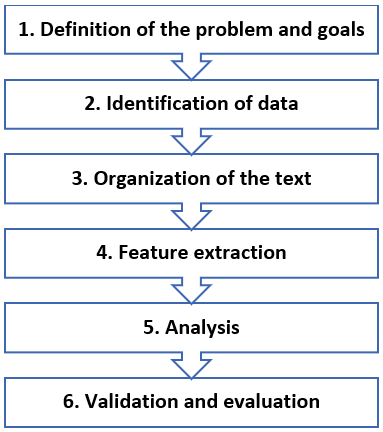
\includegraphics{images/text_mining_pipeline}
      \caption{Processing pipeline of text mining}
      \label{fig:text_mining_pipeline}
    \end{figure}
  
  \subsection{Definition of the Problem and Goals}
  \label{subsec:definition_of_the_problem_and_goals}
    In the first step we have to define the problem we want to solve. According to \citeauthor{Mitchell1997} a learning problem generally reads as follows: Improve over task $T$, with respect to performance measure $P$, based on experience $E$. The goal is therefore to generalize the experience in a way that allows to improve your performance on the task \autocite[chapter~1]{Mitchell1997}. The three parameters $T$, $P$ and $E$ are described in more detail in the following.
    \begin{itemize}
      \item Task $T$
      
        The task can be formulated by a simple verbal description, e.g. “play the game backgammon” or “sort the e-mail into the categories spam and no-spam”. A more formally approach requires the exact definition of the input and the output of the task. \\
        The input could be a map or a dictionary, i.e. a set of attribute-value pairs. In relational data, each input would have the same set of attributes and therefore the same structure and length. But since there is no restriction to the input data to be homogeneous the input can be plain text as well. A possible input of natural language could be represented by a whole book, by a (web) page, by a paragraph or just by one sentence. In certain cases, even a single letter is an appropriate input, e.g. for the detection of handwritten letters. \\
        As well as for the input we need to determine the type of output we want to receive. But not only the type, also the precision in the range of values is important for the difficulty of the task. In the case of product reviews, the easiest output “good review vs. bad review” could be complicated by using the ten values of a five-star rating allowing half stars or by distinguishing between different ratings for the quality, the price-performance ratio, the delivery etc. The aforementioned examples have in common that the number of possible output values is fixed which means a classification problem is concerned, not a regression problem. In this work the focus will be set on classification tasks.
      \item Performance measure $P$
      
        The straightforward approach to create a performance measure for classification tasks would be to count the instances with the correct output and divide this number by the total number of instances. This value is called accuracy. Just as well the complementary probability for misclassified instances, called error rate, can be observed. However, there are also possibilities to weight the classifications. If there are instances that are more important than others, these instances can be multiplied or associated with a weight greater than one. Furthermore, the misclassifications can be considered separately dependent on the correct and predicted class. In spam classification, it is usually significantly worse to classify a no-spam e-mail as spam than the other way around. To map this idea, we can assign to each pair of correct and predicted class a weight value. \\
        This type of measurement is not appropriate for regression tasks. Dependent on the exactitude of the values the probability that the predicted value is exact the correct one is low. Instead of demanding an exact prediction, we can also use the difference between correct and predicted value as the performance (MAE) or the squared difference (MSE) \autocite[section~5.8]{Witten2005}. \\
        In the case of an unsupervised problem only subjective estimates can be used. The learned model and its output are evaluated by an expert, which might entail a high expenditure of time and money. \\
        The validation and evaluation techniques will be dealt with in detail in section~\ref{subsec:validation_and_evaluation}.
      \item Experience $E$
      
        The experience of a learning problem is the knowledge the learner already possesses before solving the task. For example, a student solves exercises to gain experience before writing an exam. In machine learning, the experience is achieved through the acquisition of knowledge from databases. In both cases the learner tries to improve the performance in the task by the usage of the knowledge of similar data. If no similar data is already known, the learner can just guess the correct output. For this reason, a sufficiently large amount of data should be available to the learner in order to increase the experience and therefore also the chance to solve the task in the desired manner.
    \end{itemize}
    The following sections describe the procedure as generally as possible; we only assume that we face a classification problem in the field of text mining. Furthermore, the output value should be known for all instances, such that tasks of supervised learning can be applied automatically. As the input we use a document $d\in\mathbb{X}$, where $\mathbb{X}$ is the document space; and as the output a fixed set of classes $\mathbb{C}=\left\{c_{1},c_{2},\dots,c_{J}\right\}$. Using a learning method or learning algorithm, we then wish to learn a classifier or classification function $\gamma$ that maps documents to classes, i.e. $\gamma:\mathbb{X}\rightarrow\mathbb{C}$ \autocite[section~13.1]{Manning2008}.
  
  \subsection{Identification of Data}
    In the second step we need to find one or several data sources that offer an adequate number of instances, i.e. data sets of the previously defined input and output type. There are four characteristics to be aware of:
    \begin{itemize}
      \item Completeness
      
        Each instance of the data should be complete, i.e. we know the input and the output of the instance. All attributes of the input should be filled with a value. If they are not filled, a default value can be used or another way how to manage missing values needs to be defined. Of course, there is also a need of the completeness of the output value. Otherwise, the instance cannot be used for training nor for the evaluation.
      \item Format
      
        In addition to the completeness, the data needs to be in the same format. Using data from data sources with different syntactical structure requires a pre-processing, such that the data can be compared and processed in a similar way in further steps. This involves the order and the atomicity or distribution of the data.
      \item Quantity
      
        To be able to discover meaningful knowledge, we need a minimal data volume, usually starting from several hundreds or thousands of instances. This concerns also the absolute and the relative amount for each class or even for the most important attribute values. An upper limit of instances does not exist. However, sufficient computing and storage capacities must be available.
      \item Quality
      
        The quality of the data goes along with the completeness, but it goes one step further. The desired values should not only be existent but also accomplish quality requirements, such as observing minimal and maximal values (numeric attributes) or lengths (linguistic attributes), providing a minimal precision or being available in a specific language. Analogous to checks and other constraints in databases, the data could be validated before using it in the mining process.
    \end{itemize}
    After completing the second step we end up with an appropriate data set for the task defined in the first step. The data is in a homogeneous representation, but not necessarily in a structured form.

  \subsection{Organization of the Text}
    A big part of all data in the internet exists in the form of natural language. Usually, it is hard to evaluate the information contained in this data, because it is not structured in the same way. For example, in product reviews every customer can write his comment in a different kind, so that there is neither a certain order of the information nor a specification, which information the comment should provide. However, on the basis of an additional star rating it is possible to get a fast assessment of the customer’s attitude towards the product. So, if there is a need of further evaluation, it is helpful to have the data in a structured form instead of an unstructured form. \\\\
    Often it is not desirable or even impossible to get the unstructured data directly in a structured form, so we have to do the transformation on our own. This process of converting the data from an unstructured into a structured form is called information extraction. It is assumed that the input data is a single string, i.e. a sequence of characters. The sequence can contain just a few characters (e.g. tweets, comments) or thousands of characters (e.g. book contents). Even if in the most common cases this string is natural language, the procedure is similar for other input strings as well. In order not to falsify the data, we have to take into account the character encoding. The goal of this step is to reorganize the input from a string to a collection of tokens, also known as lexing or tokenization. This process takes place in three sub-steps:
    \begin{itemize}
      \item Token Identification
      
        A lexical token, shortly token, is a string with an identified meaning. The input string is split into substrings where each substring without meaning is discarded and all others are stored as tokens. The definition of a token depends on the use case. In natural language processing, the standard approach is to use blanks or other whitespace characters and interpunctuation symbols as separators of tokens. As a result, there are words as tokens. This general solution can be customized by interpreting whitespace characters and interpunctuation symbols (or combinations of them) as tokens. Words can also be further split at a hyphen or split into characters. The other way around, two or more words can be combined to one token, e.g. for names of persons or places (“New York”) or for usual phrases (“and so on”). All of the parts of the string that do not contain any information should be removed directly. Frequently used words as “and” or “that”, also called stopwords, do not provide added value and can be removed from the token collection. There are lists of stopwords available for common textual resources, but they may be customized for specific data sets. Other challenges in natural language processing include handling spelling mistakes, acronyms and special characters such as smileys \autocite{Kharde2016}.
      \item Normalization
      
        In this step we want to find tokens that should be treated as identical, even if the strings of the token are different. In the simplest case we can make the interpretation of a token case-insensitive by converting all occurrences into lowercase. Before doing so it should be ensured that no information is lost as a result. In sentiment analysis, a large proportion of uppercase letters could indicate rage. Other types of normalization are lemmatization and stemming. Words in natural language can be modified by inflection, most of all by conjugation (modification of verbs caused by person, tense etc.) and declination (other part of speech caused by case, gender, number etc.). Lemmatization brings all parts of speech back into its basic form, e.g. the singular nominative case for nouns or the infinitive for verbs. Stemming reduces all words independent of its part of speech to the word stem, which need not be a proper word. Though, as a consequence information about the original token get lost which can lead to incompatibilities with the further analysis in the next steps. Obviously, the order of normalization and token merging or deletion from the first step may influence the result as well and should therefore be made consciously. Besides, not only the input, but also the output can be normalized. The merging of two or more output values to one joint class can also be considered as a normalization step.
      \item Categorization
      
        This step deals with the syntactic and the semantic analysis of the tokens. Syntactic analysis, also known as parsing, is the process of assigning each token a category describing its function in the context. In classical parsing of code files, categories can be identifiers, keywords, literals etc., in parsing of natural language resources, categories can be nouns, verbs, adjectives etc. Last-mentioned is known as part-of-speech-tagging (POS-tagging). Building on the syntactic analysis we can also assign a meaning to the token in addition to the category. This process is called semantic analysis and can cover difficulties of synonyms and polysemes (ambiguous words). These semantical relations and more for English vocabulary are provided by the lexical database WordNet\footnote{\url{https://wordnet.princeton.edu/}}.
    \end{itemize}
    After finishing the chosen approaches of those three steps, we obtain the unstructured text data in a structured collection of tokens, possibly extended or replaced by their category or meaning. By splitting the string into tokens in the beginning, the tokens in the collection will be sorted in the same order as they occur in the input. The collection is in list form and the order is maintained. If the order and the count of tokens is irrelevant for further evaluation, a set can be used instead of a list. However, in most cases just the order is irrelevant but not the count of tokens, such that a multiset is the suitable form of collection. This multiset is known as “bag of words”.
  
  \subsection{Feature Extraction}
    Based on the created output from the text organization step, now the characteristics of the input data are to be figured out by feature extraction. The idea is to calculate various scores, such that we can compare the input data instances with each other, especially concerning the sentiment and polarity. At the end of this step we want to obtain a representation that can be passed as a training set to learning algorithms. \\\\
    The default feature extraction approach is typically used in web search engines during the indexing step in information retrieval. The input is a list of documents in bag of words-representation or something similar. This results in a document-term-matrix, where each row describes a document and each column the count of a specific term. This concept can be generalized and transferred to our question. The column remains the description of the document as a vector whereas each column is the value of a specific feature. The model is called Vector Space Model (VSM) as it represents each document as a vector of features which simplifies the comparison of two documents by cosine similarity. Possible features with direct relation to the token are:
    \begin{itemize}
      \item binary indication
      
        This feature holds the value 0, if the token does not occur, and the value 1 otherwise. This value follows immediately if the collection is represented as a simple set.
      \item term frequency (TF)
      
        This feature holds the count of the token as described in the information retrieval example. This value follows immediately if the collection is represented as a multiset. The value can be normalized by dividing it by the total number of tokens in the document. Another option is to relativize very high term frequency values by using the logarithm function.
      \item term frequency – inverse document frequency (TF-IDF)
      
        In contrast to the term frequency, TF-IDF decreases the weight by taking into account the number of documents in which a token appears. The idea is to reward rarely occurring tokens with a high feature value. If the token appears in all documents, the value will be 0. If the token appears in just one document, the value is maximal.
    \end{itemize}
    Features need not be dependent of only one token. There are more advanced features that use accumulation of several tokens like the average token length. The above-mentioned values can also all be calculated if the tokens are grouped by category \autocite{Wang2010}. For problems concerning long input texts in natural languages like author detection another appropriate feature is the lexical diversity. It calculates the ratio between the count of distinct words (vocabulary) and the total word count. \\\\
    If the collection is passed in list representation, we can additionally create features by using combinations of sequential tokens. These sequences are called n-grams in general; 2-grams (bigrams) and 3-grams (trigrams) are particularly frequently used. With n-grams, the context also flows into the analysis, which is an advantage, for example, when recognizing negations (“not”, “good” vs. “not good”). \\\\
    It makes sense to find in the first step as much features as possible while the computing and storage capacities are not exceeded. Thus, we get a large amount of potentially informative features. However, before passing the feature data to the learning algorithm, the dimension should be reduced to avoid redundancy and to accelerate the learning process. This step called feature selection is of particular importance for classifiers that, unlike Naïve Bayes, are expensive to train. Second, feature selection often increases classification accuracy by eliminating noise features. A noise feature is one that, when added to the document representation, increases the classification error on new data. Such an incorrect generalization from an accidental property of the training set is called overfitting \autocite[section~13.5]{Manning2008}. \\\\
    Selecting a subset of features requires a measurement value to compare the utilities of the features. Typical methods are Gini index, information gain, mutual information, $\chi^2$ or frequency-based feature selection \autocite[section~2.1]{Aggarwal2012}. All of those methods are greedy, which can lead to redundant features. There are non-greedy methods that avoid redundancy, but they are rarely used in practice due to increased computing effort \autocite[section~13.5]{Manning2008}. Finally, regardless of the choice of measurement features the features can be selected if they exceed a threshold value or all features are ranked and the best $n$ features are selected. \\\\
    A different approach for representing text data are word embeddings. The previous approaches are based on the one-hot representation: the feature vector has the same length as the size of the vocabulary. Besides the already mentioned problems due to less meaningful features and overfitting, in a one-hot representation the model cannot handle words that do not appear in the labeled training data \autocite{Turian2010}. In contrast to this, word embeddings offer a distributed representation which is dense, lowdimensional, and real-valued. They are learned on a big general corpus and can therefore associate each word with a corresponding vector. The combination of those vectors yields the document vector. The features and advantages of word embeddings have already been discussed in section~\ref{subsec:word_embeddings}.

  \subsection{Analysis}
  \label{subsec:analysis}
    In the previous chapter, the data was prepared so that we can now apply analysis procedures to the data in vector representation. The goal of this step is to find characteristics, dependencies and rules to be able to make predictions for new input data. In figure~\ref{fig:learning_approaches_sentiment_analysis} there are some possible approaches listed that can be applied to sentiment analysis problems. They can be divided into the two techniques of machine learning approaches and lexicon-based approaches \autocite{Kharde2016}.
    
    \begin{figure}[H]
      \centering
      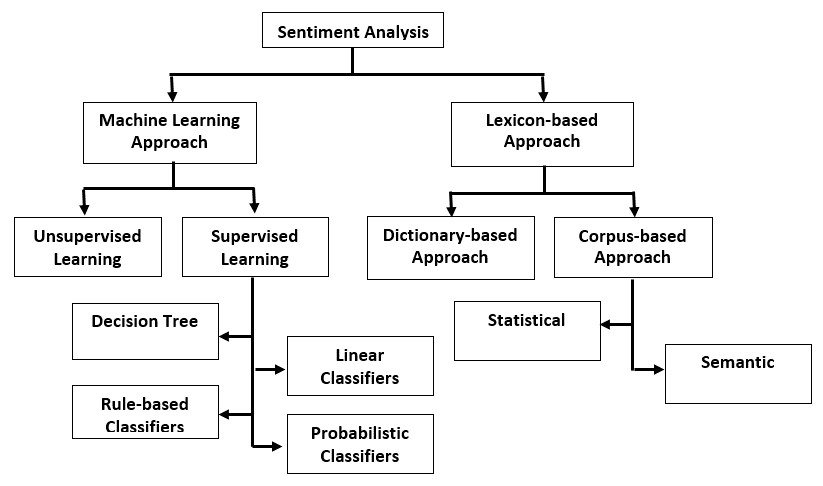
\includegraphics[scale=0.5]{images/learning_approaches_sentiment_analysis}
      \caption[Learning approaches for sentiment analysis]{Learning approaches for sentiment analysis \autocite{Halibas2018}\protect\footnotemark}
      \label{fig:learning_approaches_sentiment_analysis}
    \end{figure}
    
    \footnotetext{\url{https://www.researchgate.net/figure/Sentiment-Analysis-Source-4-Fig-1_fig1_324360275}, (11.04.2019, 23:43)}
    
    Machine learning approaches use mathematical models built by an artificial intelligence to solve the task given to them. They are split into unsupervised and supervised learning. In unsupervised learning no label of a class is provided, so there is no possibility to compare the calculated solution with the correct one. In this case a common learning approach is clustering. The input data is segmented into a (fixed) number of groups, where instances within a group should have similarities and thus form a category. In contrast, there are procedures that are to determine an output value for a given input. These are in the area of supervised learning. While regression methods can handle the assignment of continuous values, classification methods can only be applied if there is a limited and fixed number of possible output values, known as classes. \\\\
    We already defined the domain and codomain of a classification function $\gamma:\mathbb{X}\rightarrow\mathbb{C}$ where $\mathbb{X}$ is the set of documents and $\mathbb{C}$ the set of classes. Irrespective of the choice of classification algorithm, it is recommended to split the evaluation of the procedure into a training set and a test set. Based on the training set, a model can be created that learns the characteristics of a class. Partly the training set is further subdivided, whereby a model is created on the first part of the training set and fine-tuning is performed by the second part of the set (validation set). During the evaluation the correct classes of the test instances are removed. Without prior viewing, now new classes are assigned to these instances by the learned model, which are then compared with the correct classes. If, as in the case described, only one class is assigned to each instance, it is the hard version of classifying. On the contrary, the soft version assigns to an instance a probabilistic value for each class \autocite{Aggarwal2012}. In the following some such classification learning approaches are introduced, which can be used in the area of text mining:
    \begin{itemize}
      \item Decision Trees
      
        Decision trees are designed with the use of a hierarchical division of the underlying data space with the use of different (text) features. From top to bottom, the partitions become more and more homogeneous by selection of one or several appropriate features for the decision which can be determined by measurement like information gain or Gini coefficient. This procedure can be continued until all leaves are partitions containing only one class. To avoid overfitting and reduce complexity, scarcely informative sections of the tree can be cut by pruning. Finally, a test instance is associated to the class of the partition the decision path starting from the root leads to.
      \item Pattern- or Rule-based Classifiers
      
        Rule-based classifiers are similar to decision trees; more precisely, decision trees can be represented as a set of rules. For each rule the left-hand side is a condition on the underlying feature set (usually expressed in Disjunctive Normal Form (DNF)), and the right-hand side is the class label. A rule should have a high support (absolute number of instances affected by the condition) as well as a high confidence (probability for class if condition is given). In text mining, the rule is typically expressed as a conjunction of terms that have to appear in the instance. The absence of terms is rarely used, because such rules are not likely to be very informative for sparse text data. For any test instance the class of the first rule where the condition is fulfilled will be assigned. That is why the last rule should cover all remaining instances and provide a default class.
      \item Probabilistic Classifiers
      
        Probabilistic classifiers like Bayesian classifiers calculate for each class a probability, whereby the class with the highest value is chosen for the test instance. Naïve Bayes classifiers use therefore the product of all conditional probabilities, e.g. term occurrences in different classes of texts. In comparison to other classifiers, Naïve Bayes classifiers are highly scalable because of its linear complexity. Suitable probabilistic classifiers for text mining are the Bernoulli variate model and multinomial distributions.
      \item SVM Classifiers
      
        Support-vector machines (SVM) are a subgroup of linear classifiers. A linear classifier calculates for a binary classification problem a linear predictor $p= \mathbf{a}\cdot\mathbf{x}+b$, where $\mathbf{x}=(x_{1}...x_{n})$ is the feature vector of the input, $\mathbf{a}=(a_{1}...a_{n})$ is a vector of linear coefficients with the same dimensionality as the feature space and $b$ is a displacement constant. A natural interpretation of the linear predictor in the discrete scenario would be as a separating hyperplane between the different classes. The hyperplane with the maximum distance value to any instance, i.e. the one with the maximum margin of separation, is chosen. The SVM approach is quite robust to high dimensionality and ideally suited for text data because of the sparse high-dimensional nature of text \autocite{Joachims1997}.
      \item Neural Network Classifiers
      
        Simple neural networks are also a form of linear classifiers, since the function computed by a set of neurons is essentially linear. The simplest form of neural network, known as the perceptron (or single layer network) are essentially designed for linear separation, and work well for text. However, by using multiple layers of neurons, it is also possible to generalize the approach for non-linear separation. In such a network, the outputs of the neurons in the earlier layers feed into the neurons in the later layers. The training process of such networks is more complex, as the errors need to be back-propagated over different layers.
      \item Proximity-based Classifiers
      
        Those classifiers use proximity measures for classification. Given $n$ input attributes, all training instances are placed in a $n$-dimensional space. The proximity of two documents can be calculated by distance measurements like Euclidian or Manhattan distances. Then, the most common $k$-nearest-neighbor classifier identifies for a given test instance the $k$ training instances with the smallest distance values. The most common or highest-weighted class among them becomes the class of the test instance.
    \end{itemize}
    In the simplest version all of the six classifier types are applied to binary classification problems. If there are three or more classes, the classifier possibly has to be extended to handle this multiclass problem, e.g. for SVM Classifiers. Another possibility is to split the multiclass problem into several binary problems as seen in section~\ref{subsec:multiclass_classification}. The classification is made by several classifiers that are trained to differentiate either between one class and the rest (one-against-all) or pairwise between each two classes (one-against-one). Further concepts for the customization of classifiers are boosting and bagging, the formation of ensembles or the handling of ordinal classes \autocite{Aggarwal2012}. \\\\
    For sentiment analysis problems, apart from machine learning approaches also lexicon-based approaches are suitable. Lexicon-based approaches mainly rely on a sentiment lexicon, i.e., a collection of known and precompiled sentiment terms, phrases and even idioms, developed for traditional genres of communication. To determine the polarity score of a text, the polarity scores of the terms are combined in a certain way, e.g. by addition. There are two subtypes of lexicon-based approaches. The dictionary-based approach uses a list of terms called dictionary, where the collection and scores are both created manually. Manual creation may be time-consuming, but it is usually possible to create optimally customized dictionaries with good results. The corpus-based approach uses already existent dictionaries of a specific domain, which have been constructed based on a big corpus. There are statistic techniques like latent semantic analysis (LSA) as well as semantic techniques using synonyms, antonyms or other relationships from thesaurus like WordNet \autocite{Kharde2016}.

  \subsection{Validation and Evaluation}
  \label{subsec:validation_and_evaluation}
    The final step deals with the validation and evaluation of the results obtained from the previous analysis step. In section~\ref{subsec:definition_of_the_problem_and_goals} some performance measurements already have been presented. In the following only measurements for classification problems are discussed. Before discussing about those measurements, first of all we will specify how to arrange the data meaningfully to be able to perform most of the measurements. \\\\
    We already mentioned that for the evaluation the data should be split into a training and a test set. Formally speaking, a training set $\mathbb{D}$ of labeled documents $\langle d,c\rangle$ is given, where $\langle d,c\rangle\in\mathbb{X}\times\mathbb{C}$. For all unlabeled documents $d$ in the test set, the chosen classification function(s) $\gamma$ has to predict a class $c$ \autocite[section~13.1]{Manning2008}. Generally, the larger the training set the better the classifier, although the returns begin to diminish once a certain volume of training data is exceeded. And the larger the test set, the more accurate the error estimate. There are different approaches to deal with this problem \autocite[chapter~5]{Witten2005}:
    \begin{itemize}
      \item Holdout Method
      
        The simplest approach is to determine a specific percentage that should be used for training (usually two thirds). The rest of the data is cut and hold out for the final validation of unseen data. Note that here data can either be used for training or for testing.
      \item k-Fold-Cross-Validation
      
        The cross-validation tries to get away from wasting data by using all data both for training and for testing in different iterations. The data is split into $k$ folds (usually 10); $k-1$ of them are used for training and the remaining one for validation. The final measurement is the average of the measurement of all $k$ iterations and should outbid the simple holdout method in the performance value as well as in its accuracy. A non-random decomposition into folds, e.g. by previous sorting of the data records, can falsify the results.
      \item Leave-One-Out-Validation
      
        For even smaller data sets the leave-one-out-validation is a suitable approach. Here only one test instance is validated while the rest is used for training. This results in $n$ possible iterations where $n$ is the size of the data set. Similar approaches for small data sets with even more possible iterations are the leave-k-out-validation ($\binom{n}{k}$ possiblities) and the bootstrap method \autocite[chapter~4]{Arlot2010}.
    \end{itemize}
    Of course, it could be also possible not to distinguish between training and test data, i.e. the model is built and evaluated based on all data. However, this approach can lead to overfitted and therefore overestimated performance values that generally cannot be sustained in real application cases when predictions have to be made for unseen data. \\\\
    The accuracy has already been presented as a simple yet meaningful measurement value. Before it is calculated, a confusion matrix $M$ is usually created, where a value $M_{ij}$ specifies how many instances of the class $i$ were classified as class $j$. The accuracy is the sum of all values in the main diagonal of the confusion matrix (i.e. $i=j$) divided by the total number of instances. \\\\
Instead of using an absolute accuracy value it can make sense to use a relative one. In classification problems a baseline can be used as a comparison value for the accuracy. \citeauthor{Witten2005} use an expected value calculated by a default classifier as shown in table~\ref{tab:actual_and_expected_outcomes_of_three_class_classification}. They assume that the comparison classifier predicts each individual class with the same frequency as the original one. This classifier predicts for $60+18+4=82$ instances the correct class, while the original does for $88+40+12=140$. This results in $140-82=58$ additional correct classifications out of $200-82=118$ and a kappa statistic of $58\div118=49.2\%$. Another meaningful value to compare is the baseline accuracy, which is achieved by a classifier always selecting the most frequently occurring class. In the example above the baseline classifier achieves $100$ correct classification which would decrease the kappa statistic to $40\%$. Obviously, a kappa statistic of $100\%$ would indicate a perfect classifier, a value of $0\%$ no improvement and a negative value even a deterioration.
  
    \begin{table}[H]
      \subfloat[actual]{
      \begin{tabular}{cc|c|c|c|c|l}
        \cline{3-5}
        & & \multicolumn{3}{ c| }{Predicted class} \\ \cline{3-6}
        & & a & b & c & Total \\ \cline{1-6}
        \multicolumn{1}{ |c  }{\multirow{3}{*}{Actual class} } &
        \multicolumn{1}{ |c| }{a} & 88 & 10 & 2 & 100 & \\ \cline{2-6}
        \multicolumn{1}{ |c  }{} &
        \multicolumn{1}{ |c| }{b} & 14 & 40 & 6 & 60 & \\ \cline{2-6}
        \multicolumn{1}{ |c  }{} &
        \multicolumn{1}{ |c| }{c} & 18 & 10 & 12 & 40 & \\ \cline{1-6}
        \multicolumn{1}{  c  }{} &
        \multicolumn{1}{ |c| }{Total} & 120 & 60 & 20 & 200 & \\ \cline{2-6}
      \end{tabular}
      }
      \quad      
      \subfloat[expected]{
      \begin{tabular}{cc|c|c|c|c|l}
        \cline{3-5}
        & & \multicolumn{3}{ c| }{Predicted class} \\ \cline{3-6}
        & & a & b & c & Total \\ \cline{1-6}
        \multicolumn{1}{ |c  }{\multirow{3}{*}{Actual class} } &
        \multicolumn{1}{ |c| }{a} & 60 & 30 & 10 & 100 & \\ \cline{2-6}
        \multicolumn{1}{ |c  }{} &
        \multicolumn{1}{ |c| }{b} & 36 & 18 & 6 & 60 & \\ \cline{2-6}
        \multicolumn{1}{ |c  }{} &
        \multicolumn{1}{ |c| }{c} & 24 & 12 & 4 & 40 & \\ \cline{1-6}
        \multicolumn{1}{  c  }{} &
        \multicolumn{1}{ |c| }{Total} & 120 & 60 & 20 & 200 & \\ \cline{2-6}
      \end{tabular}
      }      
      \caption[Outcomes of three-class-classification]{Outcomes of three-class-classification, cf.\autocite[section~5.7]{Witten2005}}
      \label{tab:actual_and_expected_outcomes_of_three_class_classification}
    \end{table}
      
    In the kappa statistics just presented it is assumed that all false classifications are equally weighted. However, there are also cases where a classifier with negative kappa statistics is preferable to a baseline classifier. Medical classifications of patients into the classes healthy and sick are a prime example of this. A classifier with $98\%$ accuracy caused by $2\%$ of false positives (healthy patients misclassified as sick) is usually preferable to the baseline classifier with $99\%$ accuracy and the only output healthy and therefore $1\%$ of false negatives (sick patients misclassified as healthy). This is because in this case false negatives weigh heavier than false positives. For this reason, in cost-sensitive classification problems the exact cost factors for each cell in the confusion matrix have to be defined before determining a baseline classifier and an appropriate kappa statistic. In ordinal classification problems the baseline classifier with minimal costs might have the average class as the only output instead of the most common class. The influence of costs in cost-sensitive learning have already been discussed in section~\ref{subsec:cost_sensitive_learning}. \\\\
    Apart from the accuracy there are further measurement values like recall and precision. Given the confusion matrix $M$, precision and recall are defined as
    \[precision_{i}=\frac{M_{i i}}{\sum_{j}M_{ji}} \quad \textrm{and} \quad recall_{i}=\frac{M_{i i}}{\sum_{j}M_{ij}}\]
    The precision thus describes how high the quota of correctly classified instances is among all instances classified as class $i$, while the recall describes the quota of correctly classified instances among all instances that actually belong to class $i$. In binary classification problems, the formulas are simplified into
    \[precision=\frac{tp}{tp+fp} \quad \textrm{and} \quad recall=\frac{tp}{tp+fn}\]
    where $tp$ is true positives, $fp$ false positives and $fn$ false negatives. Precision and recall generally have a negative correlation and cannot be optimized at the same time. As a compromise the F-measure can be used which forms the harmonic mean of precision and recall:
    \[F=2\cdot\frac{\text{precision}\cdot\text{recall}}{\text{precision}+\text{recall}}\]
    The Receiver Operating Characteristic (ROC) is an alternative to the precision and recall measurement which visualizes the ratio of true and false positives. The confusion matrix provides only one single point for a classifier, which is generally the better the closer it is to the optimal point $(0|1)$. This point indicates $0\%$ false positives and therefore $100\%$ true negatives and optimal precision as well as $100\%$ true positives and therefore $0\%$ false negatives and optimal recall. Because false positives and false negatives can be weighted differently, the Euclidian distance has to be adjusted by different weights for the $x$- and $y$-direction. If the output values of a classifier are ranked (e.g. by probability or relevance), a whole ROC curve can be created
    \begin{itemize}[noitemsep]
      \item starting at the point (0|0),
      \item moving $\frac{1}{P}$ unit to the top in case of a true positive (where $P$ is the total number of positives),
      \item moving $\frac{1}{N}$ unit to the right in case of a false positive (where $N$ is the total number of negatives)
      \item and ending at the point (1|1).
    \end{itemize}
    In this case, the Area Under ROC Curve (AUC) is another possible indicator for a good classification. It also has a nice interpretation as the probability that the classifier ranks a randomly chosen positive instance above a randomly chosen negative one. Although those definitions and interpretations only work for binary classification problems, there are customized variants for multiclass classification, see \autocite{Hand2001}.

  \clearpage
  
  \section{Experimental Setup}
  \label{sec:experimental_setup}
    In this chapter we consider the general problem described in the previous chapter this time in the field of chess annotations. Therefore, in the beginning of this chapter, the basic chess game format PGN and the corresponding annotations NAGs are introduced. Afterwards we will follow the six steps on which the process is based on. In the following all necessary definitions and tools are presented and some statistics of the data are given. The results of the analysis and their evaluation are discussed in chapter~\ref{sec:evaluation_of_results}.
    
  \subsection{Problem Description}
    Chess games can be recorded in plain-text-files with the aim of reviewing and analyzing the game later on. Especially in professionally chess tournaments it is common to note not only the player data and the moves, but also some additional information about the game dynamics like an interim position or decisive good or bad moves. There are two ways to describe these game dynamics and annotate the chess game; either by comments in any natural language or by standardized codes and symbols like NAGs. Combinations of both variants are also common. \\\\
    For the evaluation of chess games and their machine processing the unified and structured form given by the standardized codes and symbols is preferable to the unstructured form of the comments in natural language. For chess games which only contain annotations in commentary form, it would therefore be helpful to also provide them with standard codes. This results in the problem of converting the comment into an appropriate code. Using the scheme of \citeauthor{Mitchell1997} presented in section~\ref{subsec:definition_of_the_problem_and_goals}, we have:
    \begin{itemize}[noitemsep]
      \item Task $T:$ determine the correct standard code for a given chess annotation comment
      \item Performance measure $P:$ percentage of correctly assigned codes in all code assignments (accuracy)
      \item Experience $E:$ database with tuples of comments and correct codes
    \end{itemize}
      
	\begin{figure}[H]
	  \centering
      \lstset{commentstyle=\color{blue},morecomment=[s]{\{}{\}},moredelim=[is][\bfseries]{\\textbf\{}{\}},moredelim=[is][\color{red}]{\\nag\{}{\}}}
	  \begin{lstlisting}	  
[Event "Deutschland "]
[Site "?"]
[Date "1995.??.??"]
[Round "?"]
[White "Lutz, Ch"]
[Black "Kramnik, V."]
[Result "0-1"]
[ECO "B33"]
[PlyCount "70"]
[EventDate "1995.??.??"]

\textbf{1. e4} {B33: Sicilian: Pelikan and Sveshnikov Variations} \textbf{1... c5 2. Nf3 Nc6 3.
d4 cxd4 4. Nxd4 Nf6 5. Nc3 e5 6. Ndb5 d6 7. Bg5 a6 8. Na3 b5 9. Nd5 Be7 10.
Bxf6 Bxf6 11. c3 O-O 12. Nc2 Bg5 13. a4 bxa4 14. Rxa4 a5 15. Bc4 Rb8 16. b3 Kh8
17. O-O g6 18. Qe2 Bd7 19. Rfa1 19... Bh6} {last book move} \textbf{20. g3} {
Consolidates f4} (20. Nde3 20... Be6 \nag{$14}) \textbf{20... f5} \nag{$11} \textbf{21. exf5 gxf5 22. b4
22... e4} {Black wins space.} \textbf{23. bxa5 Ne5 24. Rb4 Rxb4 25. cxb4 f4 26. Nd4 e3
27. fxe3} (27. Nxf4 \nag{$2} {doesn't work because of} 27... exf2+ 28. Qxf2 28... Bxf4
\nag{$19}) \textbf{27... f3} {He broke from his leash} (27... fxg3 28. hxg3 Qg5 29. Kh2 Nxc4
30. Nf4 \nag{$19}) \textbf{28. Qa2 f2+ 29. Kg2 Qe8 30. Be2 30... Ng4} {
The pressure on the isolated pawn grows} \textbf{31. Bf3} \nag{$4} (31. Qd2 Qh5 32. Bxg4 Qxg4
33. Nf4 Bxf4 34. exf4 Qh3+ 35. Kxf2 Qxh2+ 36. Ke1 Qxg3+ 37. Kd1 Qg1+ 38. Ke2
Bg4+ 39. Kd3 Qxa1 40. f5 \nag{$19}) \textbf{31... Nxe3+} \nag{$19} \textbf{32. Nxe3 Qxe3 33. Qxf2} \nag{$4} {
sad, but how else could White save the game?.} (33. Rd1 Bg7 34. Qb3 Bxd4 35.
Qxe3 Bxe3 36. Be2 \nag{$19}) \textbf{33... Bh3+} \nag{$1} {the final blow} \textbf{34. Kg1} {
Black now must not overlook the idea Re1} (34. Kxh3 {A deflection} 34... Qxf2)
\textbf{34... Qc3 35. Re1 Bd2} (35... Bd2 36. Ne2 36... Qxf3 \nag{$19} (36... Bxe1 \nag{$6} {
is clearly weaker} 37. Nxc3 Bxf2+ 38. Kxf2 \nag{$19}) (36... Rxf3 \nag{$2} 37. Nxc3 Rxf2
38. Kxf2 Bxc3 39. Re7 \nag{$18})) \textbf{0-1}
	  \end{lstlisting}	  

      \caption{Sample PGN game}
      \begin{tabular}{r@{: }l r@{: }l r@{: }l}
        blue & comments & red & NAGs & bold & game moves
      \end{tabular}
      \label{fig:sample_pgn_game}
	\end{figure}
	
    Before further specifying the input and output of the task $T$ in section~\ref{subsec:problem_specification}, we will first take a closer look at the structure of the chess data. The data sets used for the experience $E$ will be presented in section~\ref{subsec:data_set_extraction} and the performance measure $P$ will be adapted to the problem in section~\ref{subsec:evaluation_methods}.
    
  \subsubsection{PGN Format}
    PGN is "Portable Game Notation", a standard designed for the representation of chess game data using ASCII text files. PGN is structured for easy reading and writing by human users and for easy parsing and generation by computer programs \autocite[chapter~1]{Edwards1994}. A sample game in PGN notation is shown in figure~\ref{fig:sample_pgn_game}. \\\\
    A PGN game contains first a list of tuples with general information of the game (“tag pairs”). Seven of those tags are mandatory (Seven Tag Roster: Event, Site, Date, Round, White, Black, Result), the other tags are optional. Afterwards the “movetext” section starts. The chess moves themselves are represented using SAN (Standard Algebraic Notation). A move pair (one move of white and one of black) starts with the move pair number followed by a dot and a blank, then the move of white, another blank and the move of black, e.g. 
    \begin{quotation}
      7. Bg5 a6.
    \end{quotation}    
    Each move contains the piece by a single upper-case letter except of the pawn (see table~\ref{tab:basic_chess_notations}) followed by the square the piece is moved to (see figure~\ref{fig:square_names}). Hence, the example describes the seventh move of both players in the game; white moves his dark-squared bishop to the square g5 and black moves his a-file-pawn to a6. If a piece of the opponent is placed on the destination square, this piece is captured and in the move an "x" is inserted immediately before the destination square. In this case, if the capturing piece is a pawn, the lower-case letter of the previous file of the pawn is used at the beginning of the move, e.g. "exd5". Whenever a move pair is interrupted by a comment, the move of black is prefaced by the move pair number, an ellipsis and a blank: 
    \begin{quotation}
      Nxf4 \$2 \{doesn't work because of\} 27... exf2+
    \end{quotation}
    Additionally, there are some further moves with a special notation (see table~\ref{tab:basic_chess_notations}). In cases of disambiguation of pieces, an additional letter for the file or a number for the rank is used. In summary, a move can contain between two and seven signs in SAN \autocite[chapter~8]{Edwards1994}.
	
    \begin{figure}[H]
      \begin{floatrow}
      \capbtabbox[10.4cm]{%
        \begin{tabular}{| l | l |}
    	\hline
    	Symbol & Meaning \\ \hline
    	  K & King \\ \hline
    	  Q & Queen \\ \hline
    	  R & Rook \\ \hline
    	  B & Bishop \\ \hline
    	  N & Knight \\ \hline
    	  \textit{blank} & Pawn \\ \hline
        \end{tabular}
        \begin{tabular}{| l | l | l |}
    	  \hline
    	  Symbol & Meaning & Example \\ \hline
    	  x & Capture & Rxa1 \\ \hline
    	  + & Check & Nf6+ \\ \hline
    	  \# & Checkmate & Bb7\# \\ \hline
    	  0-0 & Castling kingside & \\ \hline
    	  0-0-0 & Castling queenside & \\ \hline
    	  = & Promotion & fxg1=Q+ \\ \hline
        \end{tabular}
      }{%
        \caption{Basic chess notations}
        \label{tab:basic_chess_notations}
      }
      \ffigbox[6.6cm]{%
	    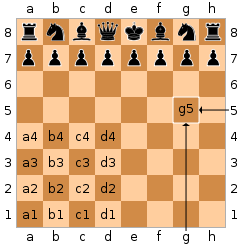
\includegraphics[scale=0.5]{images/algebraic_notation}
      }{%
	    \caption[Square names in algebraic notation]{Square names in algebraic notation\protect\footnotemark}
        \label{fig:square_names}
      }
      \end{floatrow}
    \end{figure}
    
  	\footnotetext{\url{https://en.wikipedia.org/wiki/Algebraic_notation_(chess)\#/media/File:SCD_algebraic_notation.svg}, (18.03.2019, 20:56)}
  	
	Parts of the moves are annotated using comments in braces. A comment can contain information about the opening of the game, about a single move or about the current position. In the last two cases the comment is often prefaced by one or several NAGs (see section~\ref{subsec:nags}) or the corresponding chess symbol. Since there is no restriction on the exact position of a comment, comments may refer to the move before or after itself. A comment can also connect two or more moves with each other. On the contrary, a comment can be interrupted by a move such that it is split into two parts, which may only make sense when seen together. All in all, there are four possibilities of comment-move combinations shown in the examples of table~\ref{tab:comment_move_combinations}.
	
	\begin{table}[H]
      \centering
      \begin{tabular}{| l | l |}
    	\hline
    	Combination & Example \\ \hline
    	Move, Comment & e4 \{Black wins space.\} \\ \hline
    	Comment, Move & \{Weaker is\} 39. Bxe6 \\ \hline
    	Move, Comment, Move & Nxf4 \$2 \{doesn't work because of\} 27... exf2+ \\ \hline
    	Comment, Move, Comment & \{Because of the blunder\} 24. Txf8 \{Black wins immediately\} \\ \hline
      \end{tabular}      
      \caption{Comment-move combinations}
      \label{tab:comment_move_combinations}
    \end{table}
    
    Besides, by convention there should not be nested braces, however, sometimes nested braces are used to comment different move variants separately.	Those variants need not be part of a comment and are written down in parenthesis. The enumeration of the moves proceeds within a variant and is set back before a new variant starts or the game itself continues. 
   
  \subsubsection{NAGs}
  \label{subsec:nags}
    Numeric Annotation Glyphs (NAGs) are used to annotate chess games with assessments of moves or positions in a standard way. They are standard annotation symbols in PGN files, but can as well be used in other chess formats. A NAG is composed of a “\$” followed by one or more digits. There are 140 standard NAGs in total:
    \begin{itemize}[noitemsep]
      \item NAG zero is used as a placeholder
      \item NAGs with values from 1 to 9 annotate the move just played.
      \item NAGs with values from 10 to 135 annotate the current position.
      \item NAGs with values from 136 to 139 describe time pressure.
    \end{itemize}
    The NAGs with values from 140 to 255 are partially defined and used unofficially. The most common NAGs are listed in table~\ref{tab:meaning_of_nags} (see \autocite[chapter~10]{Edwards1994}).
	
	\begin{table}[H]
      \subfloat[move-annotating NAGs]{
      \begin{tabular}{| c | c | l |}
    	\hline
    	NAG & Symbol & Meaning \\ \hline
    	\$1 & ! & good move \\ \hline
    	\$2 & ? & poor move \\ \hline
    	\$3 & !! & very good move \\ \hline
    	\$4 & ?? & very poor move \\ \hline
    	\$5 & !? & speculative move \\ \hline
    	\$6 & ?! & questionable move \\ \hline
      \end{tabular}
      }
      \quad
      \subfloat[position-annotating NAGs]{
      \begin{tabular}{| c | c | l |}
    	\hline
    	NAG & Symbol & Meaning \\ \hline
    	\$10 & $=$ & drawish position \\ \hline
    	\$11 &  & equal chances, quiet position \\ \hline
    	\$12 &  & equal chances, active position \\ \hline
    	\$13 & $\infty$ & unclear position \\ \hline
    	\$14 & $+=$ & White has a slight advantage \\ \hline
    	\$15 & $=+$ & Black has a slight advantage \\ \hline
    	\$16 & $\pm$ & White has a moderate advantage \\ \hline
    	\$17 & $\mp$ & Black has a moderate advantage \\ \hline
    	\$18 & $+-$ & White has a decisive advantage \\ \hline
    	\$19 & $-+$ & Black has a decisive advantage \\ \hline
      \end{tabular}
      }
      \caption{Meaning of NAGs}
      \label{tab:meaning_of_nags}
	\end{table}
	
	As shown in table~\ref{tab:meaning_of_nags}, the most common NAGs have a corresponding symbol, which has been used traditionally. Those symbols are composed of the signs “!”, “?”, “+”, “-“, “=” and special signs. It should be emphasized that the subjective symbols do not mix up with the objective move symbols for check and promotion because they are used in different combinations.

  \subsubsection{Problem Specification}
  \label{subsec:problem_specification}
    Now the structure of PGN chess files and the corresponding NAGs being clarified, we can identify use cases in which a sentiment analysis of chess annotations might be useful. In PGN files, comments are often assigned to the NAG that precedes this comment. If no NAG is given - which is the case for more than half of all comments (see table~\ref{tab:file_statistics}) - we could assign the correct NAG automatically if we would have a reliable learned model. Thus, we will collect the data of already correctly mapped comments and NAGs and recognize contained patterns therein. Concretely, the following problems will be discussed:
    \begin{itemize}
      \item Classification into move and position annotations

      As already seen in table~\ref{tab:meaning_of_nags}, the NAGs are subdivided into NAGs annotating moves and NAGs annotating positions (those describing time pressure are rarely used and therefore negligible). Both annotation types are used at the same place in the PGN file, in particular directly after a move. Therefore, we need to recognize and learn other patterns in order to distinguish these two types of annotations. For this learning problem, the input space $\mathbb{X}$ and output space $\mathbb{C}$ are defined as follows:
      \begin{quotation}
        $\mathbb{X}:=$ set of chess comments without annotation \quad $\mathbb{C}:=\{1,2\}$
      \end{quotation}
      The output class $1$ is used for move annotations and the class $2$ for position annotations. 
      \item Classification of move annotations

      Among the move-annotating NAGs there are basically two groups of annotations; positive and negative ones. It should be noted that positivity and negativity does not refer generally to white or black, but from the viewpoint of the player with the move directly before the NAG. We can formulate the classification problem on the same input space in two degrees of difficulty:
      \begin{quotation}
        $\mathbb{X}:=$ set of move comments without annotation \quad $\mathbb{C}_{1}:=\{1,2\} \quad \mathbb{C}_{2}:=\{1,2,3,4,5,6\}$
      \end{quotation}
      In the first output set, the class $1$ is assigned to all positive move annotations (i.e. \$1, \$3, \$5) and the class $2$ to the negative ones (i.e. \$2, \$4, \$6). In the second output set, each of the six NAGs gets an own class ranked by their “positiveness”. This converts the binary classification problem to an ordinal classification problem with the following mapping of NAGs to classes (1 = most positive, 6 = most negative):
      \begin{quotation}
        $1: \$3$ \quad $2: \$1$ \quad $3: \$5$ \quad $4: \$6$ \quad $5: \$2$ \quad $6: \$4$
      \end{quotation}
      \item Classification of position annotations

      With the position-annotated NAGs we have a similar situation, but with the decisive difference that a neutral class also exists. So even the simpler classification problem already contains three classes:
      \begin{quotation}
        $\mathbb{X}:=$ set of position comments without annotation \quad $\mathbb{C}_{1}:=\{1,2,3\} \quad \mathbb{C}_{2}:=\{1,2,3,4,5,6,7\}$
      \end{quotation}
      In the first output set, the class $1$ is assigned to all position annotations with an advantage of white (i.e. \$14, \$16, \$18), the class $2$ to the balanced position annotations (i.e. \$10, \$11, \$12, \$13) and the class $3$ to the annotations with an advantage of black (i.e. \$15, \$17, \$19). In the second output set, classes $1$ and $3$ are each divided into three subclasses, which makes a total of seven ordered classes (1 = best for white, 7 = best for black):
      \begin{quotation}
        $1: \$18$ \quad $2: \$16$ \quad $3: \$14$ \quad $4: \$10,\$11,\$12,\$13$ \quad $5: \$15$ \quad $6: \$17$ \quad $7: \$19$
      \end{quotation}
    \end{itemize}
    Note that in all cases only one of the output values can be assigned, i.e. we only face single-label problems.
  
  \subsection{Data Set Extraction}
  \label{subsec:data_set_extraction}  
    As data sources a set of files\footnote{\url{http://www.angelfire.com/games3/smartbridge/}} in standard PGN format is used as well as a bundle of commented games that have been extracted from Mega Database 2012\footnote{\url{https://shop.chessbase.com/en/products/mega_database_2012}} in ChessBase format. The related user interface ChessBase Reader offers the possibility to select the desired games and convert them into the standard PGN format. As a result, we obtain a set of files each containing several games in PGN format like seen in figure~\ref{fig:sample_pgn_game}. In total, we analyze 39 files with 68,606 games. In the next step those files have to be read and converted into data sets with comments that can be used within the classification problem. For this purpose, the natural language toolkit NLTK is used. \\\\
    NLTK\footnote{\url{https://www.nltk.org/}} is a python library offering various technique for natural language processing (NLP). It can be used to extract information from web files in html or any other text file format. Besides, it offers access to big corpora and other lexical resources. The NLP process and its corresponding code in python using NLTK is shown in figure~\ref{fig:nlp_pipeline}. Note that the pictured steps of tokenization and normalization are not considered in this section, but in section~\ref{subsec:nltk_preprocessing}.

    \begin{figure}[H]
      \centering
      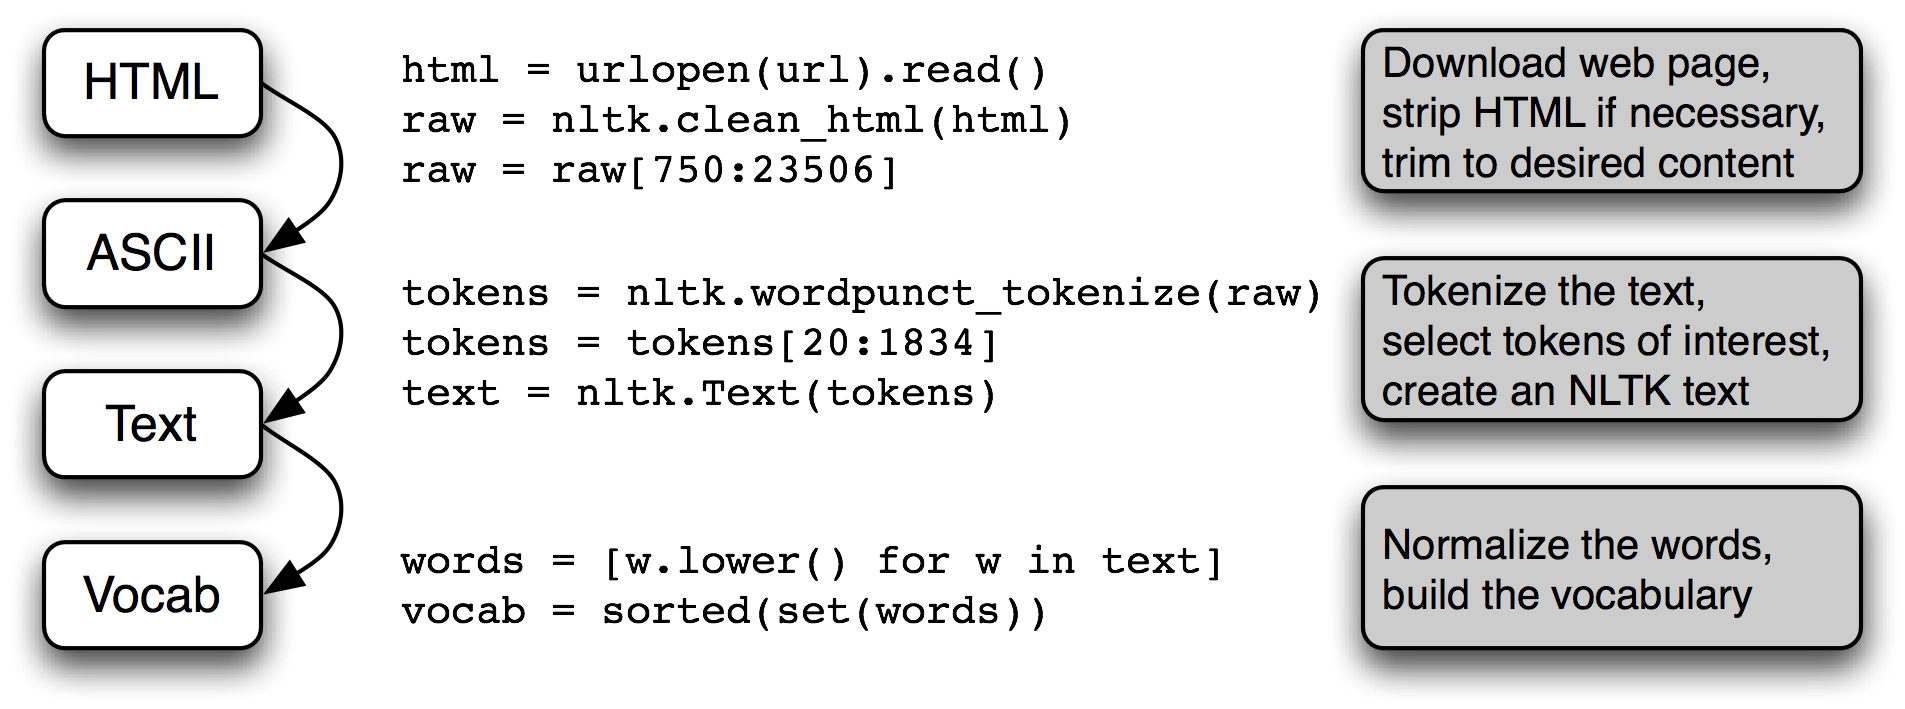
\includegraphics{images/nlp_pipeline}
      \caption[NLP pipeline]{NLP pipeline cf.\autocite[section~3.1]{Bird2009}}
      \label{fig:nlp_pipeline}
    \end{figure}
    
    Applied to the chess annotation problem, the raw text of the PGN files can be extracted and decoded by the following two commands    
    \begin{lstlisting}
    raw = open(file, 'rb').read()
    string = raw.decode('iso-8859-1')
    \end{lstlisting}  
    where the variable \textit{file} contains both the relative path and the filename. The process is repeated for each filename saved in a list. An ISO 8859-1-decoding is used instead of an ASCII-decoding to detect the Western European letters used in comments and player names correctly. \\\\
    However, we are not interested in the complete raw text of the PGN files, but only in the comments. As we have already seen in table~\ref{tab:comment_move_combinations}, there are different comments in a PGN file. Since we want to be able to use supervised learning approaches, we need to know the correct class of a comment in the file. Therefore, the comments which are from importance are those connected to a traditional chess symbol or a NAG. To filter out such comments, we use regular expressions and distinguish between three cases:
    \begin{itemize}
      \item NAGs immediately followed by a comment:

        \textbackslash\$(?P<class>[0-9]+)\textbackslash s*\textbackslash\{(?P<comment>[$\hat{}$\{\}]*)\textbackslash\}
      \item NAGs followed by another NAG and thereafter a comment:

        \textbackslash\$(?P<class>[0-9]+)\textbackslash s*\textbackslash\$[0-9]+\textbackslash s*\textbackslash\{(?P<comment>[$\hat{}$\{\}]*)\textbackslash\}
      \item Standard symbols for move annotations (i.e. $!,?,!!,??,!?,?!$) immediately followed by a comment:

        (?P<class>[!\textbackslash?]\{1,2\})\textbackslash s*\textbackslash\{(?P<comment>[$\hat{}$\{\}]*)\textbackslash\}
    \end{itemize}
    The match results are saved as tuples of the class (NAGs without dollar sign, symbols unchanged) and the comment. The final class is set depending on the rules of the considered classification problem by using a python dictionary, e.g. for the binary move annotation problem all the classes $1, 3, 5, !, !!, !?$ are mapped to the final class $1$. \\\\
    So far, we ensured the collected data to be complete (class is known), in a specific format (PGN, processed to tuple) and available in sufficient quantity. Before proceeding with the next step, we will perform some basic analysis on the extracted data to estimate the quantity of comments per class. This includes a comparison of the total count of all symbols and NAG types for every of the three tasks we specified in section~\ref{subsec:problem_specification}. If the counts would differ a lot, different weights should be assigned to the instances to avoid imbalances and thus difficulties in classification. The data shown in table~\ref{tab:class_distributions} has indeed some noticeable imbalances; instances with positive move annotations are more common than negative ones as well as surprisingly an advantage of white is more common than an advantage of black in the position annotations. However, these imbalances are in an uncritical range, which probably requires no weighting of instances.

	\begin{table}[H]
      \subfloat[all annotations]{
      \begin{tabular}{| r | r | r | r |}
    	\hline
    	Final class & Symbol \& NAGs & Count & Percentage \\ \hline
	    $1$ & all symbols, $\$1-\$9$ & $224,619$ & $44.04\%$ \\ \hline	
	    $2$ & $\$10-\$135$ & $268,060$ & $52.57\%$ \\ \hline	
	    \multicolumn{2}{ |l| }{Total} & $492,679$ & $96.61\%$ \\ \hline\hline		
	    $-$ & $\$136-\$255$ & $17,313$ & $3.39\%$\\ \hline
      \end{tabular}
      }
      \quad
      \subfloat[move annotations]{
      \begin{tabular}{| r | r | r | r |}
    	\hline
    	Final class & Symbol \& NAGs & Count & Percentage \\ \hline
	    $1$ & $!!,\$3$ & $3,226$ & $1.44\%$ \\ \hline	
	    $2$ & $!,\$1$ & $105,789$ & $47.10\%$ \\ \hline	
	    $3$ & $!?,\$5$ & $50,636$ & $22.54\%$ \\ \hline		
	    $4$ & $?!,\$6$ & $29,838$ & $13.28\%$ \\ \hline		
	    $5$ & $?,\$2$ & $28,660$ & $12.76\%$ \\ \hline	
	    $6$ & $??,\$4$ & $4,849$ & $2.16\%$ \\ \hline	
	    \multicolumn{2}{ |l| }{Total} & $222,998$ & $99.28\%$ \\ \hline\hline		
	    $-$ & $\$7-\$9$ & $1,621$ & $0.72\%$\\ \hline
      \end{tabular}
      }
      \quad
      \subfloat[position annotations]{
      \begin{tabular}{| r | r | r | r |}
    	\hline
    	Final class & NAGs & Count & Percentage \\ \hline
	    $1$ & $\$18$ & $23,500$ & $8.77\%$ \\ \hline	
	    $2$ & $\$16$ & $42,975$ & $16.03\%$ \\ \hline	
	    $3$ & $\$14$ & $53,599$ & $20.00\%$ \\ \hline		
	    $4$ & $\$10-\$13$ & $58,774$ & $21.93\%$ \\ \hline		
	    $5$ & $\$15$ & $17,841$ & $6.66\%$ \\ \hline	
	    $6$ & $\$17$ & $16,092$ & $6.00\%$ \\ \hline	
	    $7$ & $\$19$ & $11,559$ & $4.31\%$ \\ \hline	
	    \multicolumn{2}{ |l| }{Total} & $224,340$ & $83.69\%$ \\ \hline\hline		
	    $-$ & $\$20-\$135$ & $43,720$ & $16.31\%$\\ \hline
      \end{tabular}
      }
      \caption{Class distributions}
      \label{tab:class_distributions}
	\end{table}
	
    The last criterion quality will be discussed in section~\ref{subsec:nltk_preprocessing}. Possible problems are that the comment is in a different language than English or that the comment is too short to make an informed classification decision. \\\\
    Apart from the statistics on the file data to be further processed, some information about the discarded data are relevant for the usage of the results we obtain. By collecting the number of all comments not annotated with a NAG or standard symbol yet we obtain the potential of improvement regarding the comments. As shown in table~\ref{tab:file_statistics}, only $45.39\%$ of the comments are preceded by a NAG or symbol. For the remaining $54.61\%$ of the comments, which are still more than half a million, the comment could be completed with an appropriate NAG or symbol. The other way around, this approach delivers a ratio of $25.06\%$ NAGs and standard symbols that are followed by a comment. In contrast to the first case, adding a comment is not useful or necessary, while adding a NAG is usually possible for most comments except those describing general game information like opening variants or summaries.
	
	\begin{table}[H]
      \begin{tabular}{| l | r | r |}
    	\hline
    	 & Count & Percentage of processed data \\ \hline
    	Classes \& Comments & $509,992$ & $100.00\%$ \\ \hline
    	Comments & $1,123,538$ & $45.39\%$ \\ \hline
    	Classes & $2,035,121$ & $25.06\%$ \\ \hline
      \end{tabular}
      \caption{PGN file statistics}
      \label{tab:file_statistics}
	\end{table}
	
    To get the values of table~\ref{tab:file_statistics}, the number of comments is estimated by counting all occurrences of opening braces (\{), the number of NAGs by all occurrences of the dollar sign (\$) and the number of standard symbols by the number of matches of the regular expression \textbackslash d\textbackslash+*\textbackslash s*[!\textbackslash?]+ (an arbitrary combination of the symbols $!$ and $?$, preceded by the number of the move field square and optional a check(mate) symbol and whitespace. Due to this rudimental approach of counting, the expressions could also match false positives, if some of the symbols are used in a different sense. However, this number of false positives is small and therefore negligible.	

  \subsection{NLTK Preprocessing}
  \label{subsec:nltk_preprocessing}    
   The output of the previous step is a set of tuples containing the comment and the class. Since a direct evaluation of the comments is only limited possible, there is a need to split the comments into substrings with an identified meaning by tokenization. NLTK offers the method "word\textunderscore tokenize" adjusted to natural language text data in addition to the straightforward method of splitting the comment by the whitespaces. However, the use of "word\textunderscore tokenize" for punctuation symbols is not appropriate for all cases. If move variants are presented in a comment or additional NAGs are used, "word\textunderscore tokenize" may not separate them as desired. A separate handling of such tokens is possible with a regular expression tokenizer. \\\\
    The RegexpTokenizer of NLTK has a regular expression as its only parameter and splits the text into tokens using this expression. Several regular expressions can be combined by the conjunction symbol $|$. The tokenizer then takes the first of the expressions the part of the text matches, wherefore in the case of ambiguities the most specific or important expressions must be at the beginning. The parts of the text not matching any case of the regular expression are discarded. \\\\
    For the creation of a suitable regular expression tokenizer for comments in PGN files, the token definition according to PGN file specification was taken into account \autocite[chapter~7]{Edwards1994} and some comments were examined manually for their structure. This leads to a regular expression based on the following cases:
    \begin{itemize}
      \setlength\itemsep{0.4em}
      \item \makebox[7cm][l]{PGN non-standard codes} \#[\textbackslash w\textbackslash d]{2}
      \item \makebox[7cm][l]{NAG non-standard codes} \textbackslash\$\textbackslash d+
      \item \makebox[7cm][l]{Move-annotating symbols} [!\textbackslash?]+
      \item \makebox[7cm][l]{Position-annotating symbols } [\textbackslash-\textbackslash+/=]+
      \item \makebox[7cm][l]{Remis symbol} 1/2
      \item \makebox[7cm][l]{Abbreviations} (?:\textbackslash w\textbackslash.)+
      \item \makebox[7cm][l]{Multiple dots} \textbackslash.+
      \item \makebox[7cm][l]{Words (including hyphens or apostrophes)} [\textbackslash w\textbackslash d\textbackslash-\textbackslash']+
      \item \makebox[7cm][l]{Remaining non-whitespace characters} \textbackslash S
    \end{itemize}
    The first two cases match non-standardized, but nevertheless frequently used abbreviations for common chess phrases. For example, the non-standard PGN code \#C4 and the non-standard NAG $\$142$ mean “Better is…” and could indicate a suboptimal move of class $4$ or $5$. The next three cases match symbols annotating moves and positions of follow-up variants. The regular expressions for abbreviations and multiple dots should reduce the number of tokens and avoid to mix this kind of expressions with other dots. Most tokens match the regular expression for words, that does not only include words of natural language, but also numbers, chess moves and the remaining position expressions $1-0$ and $0-1$. Finally, with the last expression the remaining non-whitespace characters like punctuation symbols are fetched. Different configurations of the tokenizer will be evaluated in section~\ref{subsec:tokenizer_evaluation}. \\\\
    The normalization step is already involved in the tokenization process. Before splitting the comment into its tokens, it is already converted in lowercase, because this conversion does not influence the tokenization process. Immediately after the tokenization follows the lemmatization of the words. In this case lemmatization is preferred to stemming, because the language of lemmatized tokens can be better detected than for stemmed tokens. Besides, lemmatized tokens are easier to read than stemmed tokens. Categorization is waived, but it is implicitly used in the word embedding models, which receive the tokenized data as input later on. The normalization of the output, i.e. the conversion of the NAGs and symbols to the classes of the problem, is moved to after feature extraction and selection, because until then all comments can be processed uniformly for all problems.

    \begin{figure}[H]
      \centering
      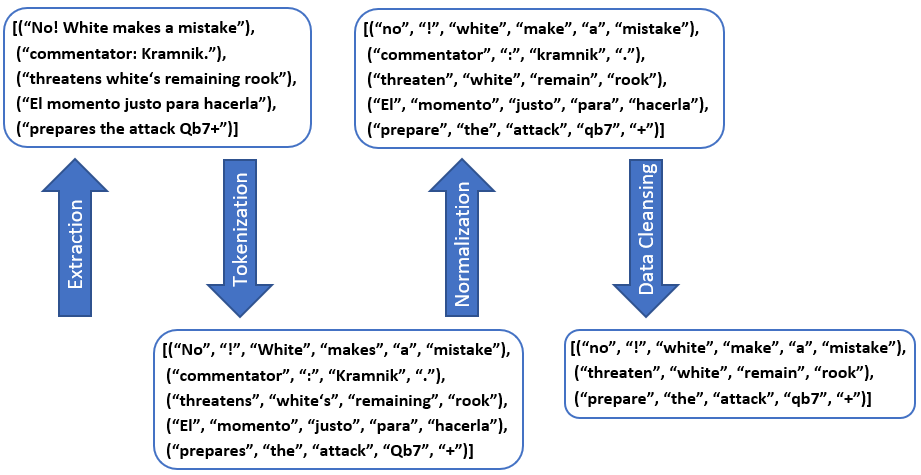
\includegraphics[scale=0.9]{images/nltk_preprocessing}
      \caption{NLTK preprocessing}
      \label{fig:nltk_preprocessing}
	\end{figure}  
    
    The tokenizer produces an ordered list of tokens as output. Before proceeding with the feature extraction and selection, we first perform the missing checks on the language and the length of the comment. Comments in different languages lead to different rules and are therefore difficult to process at the same time. Long comments often contain descriptions about openings, other variants or similar chess games and are therefore unsuitable. Comments that are too short, on the other hand, generally provide little information and are not very meaningful. Besides, comments with just one or two tokens often just contain the name of the commentator. In order to be able to make reliable classification decisions, we require at least three tokens that are part of the English vocabulary to be included in each further processed comment. Thus, a minimum length of three tokens is guaranteed as well. The maximum length should be set to 49 tokens. \\\\
    Unfortunately, it is not possible to filter the games directly in the ChessBase Reader by the used comment language. For this reason, the additional language detection library langid is used to filter out comments already before the tokenization process if with $99\%$ confidence the detected language is not English. Through this, over $70,000$ comments will be discarded. The second language detection step starts after the tokenization and normalization. For each comment the tokens are iterated and checked if the lemmatized token is part of the English vocabulary provided by the NLTK corpus. If there are at least three such words, the comment will be forwarded to the feature extraction and selection process. Although false positives cannot be completely avoided with this approach, the proportion of long comments in non-English should be low due to the first filter. Not filterable are however some comments of the ChessBase database, which contain the same statements united in several different languages. For this reason, some tokens will be in a different language than English. The complete NLTK preprocess is shown in figure~\ref{fig:nltk_preprocessing}. \\\\
    All in all, 70\% of the comments are filtered due to the above-mentioned quality requirements. 156,970 out of 511,273 comments remain, which is still sufficient data to learn on. In order to keep the computing capacities and times within reasonable limits such that different configurations can also be tested, 4,000 instances are selected, including 2,000 move annotations and 2,000 position annotations. Two more datasets of the same size are created for short comments with a token length of 3 to 9 and for long comments with a token length of 10 to 49, without overlapping with the first dataset. These three datasets are passed as a list of tuples of tokenized comments and NAGs or symbols to the feature extraction and selection step. The order of the tokens remains unchanged by selecting a list as collection type. \\\\

  \subsection{Attribute Creation and Selection}
    In this step the text instances should be converted to a vector of numbers, whereby each number represents an attribute of the comments. All these vectors are strung together in a matrix, that is passed in an appropriate format to the analysis step. First different models for the generation of attributes are introduced, before the second step describes the transformation of the model data into an ARFF file.
      
  \subsubsection{Model Generation}
In the following four different models are built in order to offer an appropriate attribute set for the analysis. The models have no attributes in common except of two; the number of tokens and the class attribute. For all models the attributes are all numeric except of the class attribute.
    \begin{itemize}
      \item Count-based Model

        The count-based model uses the CountVectorizer class of the machine learning library scikit-learn\footnote{\url{https://scikit-learn.org/stable/index.html}}. It converts the comments to a matrix of features, where each row represents a comment and each column a term of the vocabulary. The vocabulary is made up of all tokens, bigrams or trigrams that occur at least in five comments in the data set. The vectorizer counts the occurrences of each term in the vocabulary in each comment and stores the count in the corresponding cell of the matrix. As the comments are already lowercase and tokenized, these options do not have to be configured.
      \item TF-IDF-based Model

        The TF-IDF based model is similar to the count-based model, but uses the TfidfVectorizer class. The vectorizer is configured as in the first model, i.e. it builds a vocabulary of tokens, bigrams and trigrams with minimal one occurrence in five different comments. However, the matrix this time contains the relative values for the occurrences of the term. Two terms that have the same value in the count-based model now have different values if the number of documents in which the term appears varies. The more documents contain the term, the lower the value.
      \item Own Word2Vec-Model

        This model uses the word2vec module of the machine learning library gensim\footnote{\url{https://radimrehurek.com/gensim/models/word2vec.html}} to create a word embedding for chess annotations. A CBOW-word2vec-model is built and trained for all words in the chess comments. This time there is no need to include bigrams and trigrams in the model, because the context of a word is already taken into account by the window size of five. Similar to the first two models, all words with less than five occurrences are ignored and no part of the vocabulary. However, this time five is the limit for the total number of occurrences, i.e. a word only occurring in a single comment, but therein at least five times, will nevertheless be processed. As a result, the matrix contains a dense vector with 100 attributes for each word. To obtain the vector $\mathbf{v_{c}}$ for a comment $c$, the product of all vectors $\mathbf{v_{w}}$ and IDF-scores $idf_{w}$ of words $w$ in the comment that are also in the vocabulary are averaged:
        \[\mathbf{v_{c}}=\sum_{\substack{w\in c\\w\in vocab}}\mathbf{v_{w}}\cdot idf_{w}\]
        Note that the weighted vectors have to be averaged and not summed up to handle different comment lengths. The term frequency is automatically included if the comment is treated as a list.
      \item Pretrained Word2Vec-Model

        This model is as well based on word embeddings, but instead of creating a new model, an existing model is imported. It learned word vectors for all terms appearing in a huge Google News data set. It offers 300 attributes for around 3,000,000 words. Terms that are not part of the vocabulary are usually nevertheless matched by a pattern and a corresponding vector. Like in the previous case, the output matrix contains the vector of the comments in the data set, where each vector is calculated as the average of the weighted word vectors.
    \end{itemize}
    The first two models offer a large number of attributes. Even if this number is already limited by the minimal number of five occurrences in the whole data set, an upper limit of 2,000 attributes is defined to limit the computing time of the algorithms. Both for the count-based and the TF-IDF-based model, the attributes are therefore ordered by their total term frequency and the top 2,000 remain in the model. For the short comment data set there is even no attribute selection required, because the vocabulary contains only 1,631 attributes. At this point it should be noted that usually it is not recommended to apply attribute selection to all data, but only to the training data, because otherwise the test data has been seen by the attribute selection process and the accuracies are too optimistic. Due to the fact, that for the attribute selection process the class attribute is not considered, this falsification should be minimal, if any.
  
  \subsubsection{Conversion to ARFF}
    Weka\footnote{\url{https://www.cs.waikato.ac.nz/ml/weka/}}, short for Waikato Environment for Knowledge Analysis, is an open source software offering a collection of machine learning algorithms for data mining tasks that will be addressed to in section~\ref{subsec:classification_algorithms}. The algorithms are applied to data represented in Attribute-Relation File Format (ARFF)\footnote{\url{https://www.cs.waikato.ac.nz/ml/weka/arff.html}}. Weka offers standard ARFF files to experiment with and to get to know the functionality of the machine learning methods. As well own ARFF files can be imported and used. For this purpose, an ASCII text file needs to be structured as shown in figure~\ref{fig:sample_arff_files}. It shows a possible output ARFF file for the two-class move annotations problem with two comment-value-pairs (“a brilliant counterattack of white”, 1) and (“a big mistake of black”, 2). The file consists of two blocks, the header information and the data information. Before the header information there might be comment lines with information about the author and version or further descriptions.
    
    \newsavebox{\complete}
      \begin{lrbox}{\complete}
        \lstset{keywordstyle=\color{blue},keywords={@RELATION,@ATTRIBUTE,@DATA,NUMERIC,REAL}}
        \begin{lstlisting}
@RELATION comment-move-1
@ATTRIBUTE count(brilliant) NUMERIC
@ATTRIBUTE tfidf(mistake) REAL
@ATTRIBUTE class {1,2}
@DATA
1, 0.0, 1
0, 0.06, 2	  
        \end{lstlisting}      
      \end{lrbox}
    \newsavebox{\sparse}
      \begin{lrbox}{\sparse}
        \lstset{keywordstyle=\color{blue},keywords={@RELATION,@ATTRIBUTE,@DATA,NUMERIC,REAL}}
        \begin{lstlisting}
@RELATION comment-move-1
@ATTRIBUTE count(brilliant) NUMERIC
@ATTRIBUTE tfidf(mistake) REAL
@ATTRIBUTE class {1,2}
@DATA
{0 1, 2 1}
{1 0.06, 2 2}	  
        \end{lstlisting}        
      \end{lrbox}    
    
    \begin{figure}[H]
	  \centering      
	  \subfloat[complete]{\usebox{\complete}\label{fig:sample_arff_file_complete}}
	  \quad
	  \subfloat[sparse]{\usebox{\sparse}\label{fig:sample_arff_file_sparse}}
      \caption{Sample arff files}
      \label{fig:sample_arff_files}
	\end{figure}
    
    The first block of the header information contains the keyword “@RELATION” and an arbitrarily name for the relation in the first line. After that for each attribute the relation contains a triple of the keyword “@ATTRIBUTE”, a unique name of the attribute and the data type of the attribute. The data type can be numeric (integer, real), string, date or nominal. For the first three data types, only the type needs to be indicated, whereas nominal attributes require a list of all possible values comma-separated in braces. The output value of an instance is an attribute as well and need to be specified, conventionally as the last attribute. In classification problems the class attribute has a fixed number of values and is represented as nominal in the form of a set, in regression problems it is numeric. \\\\
    The second block begins with the keyword “@DATA” in the first line. After that for each instance the values of the attributes are listed comma-separated, in the same order as they were declared before, see figure~\ref{fig:sample_arff_file_complete}. Missing values are indicated by a “?”. Data sets can consist for the most part of zero values, in particular those with attributes used in Information Retrieval like TF or TF-IDF. In order to reduce the creation time and the size of the file, in sparse ARFF files (see figure~\ref{fig:sample_arff_file_sparse}) numeric values are zero by default and can be omitted. However, now the instances can consist of a different number of values. For this reason, each instance is represented as a comma-separated list of pairs, surrounded by braces. The first number of a pair is the attribute id (starting from zero), the second one the value. Missing values are not equal to zero and need to be indicated by a “?” further on. \\\\
    For the matrix output of the count and TF-IDF based model, choosing the sparse representation form significantly reduces the size of the ARFF file. Since it only requires a small additional effort for the two Word2Vec models, a uniform transformation into sparse ARFF files is executed. Such a file is thus generated for each combination of the five problems, the four models and the three data sets, so that a total of 60 files are passed on for analysis. Note that now the NAGs and symbols are converted to the corresponding class depending on the problem.
    
  \subsection{Classification Algorithms}
  \label{subsec:classification_algorithms}
    For the analysis of the data sets in the generated ARFF files the already mentioned software Weka will be used. It offers many tools to prepare, process and evaluate data by different machine learning techniques. For the purposes of this work mainly the configurations of the “Classify” tab in the Weka explorer are used as shown in figure~\ref{fig:weka_classify}.
        
    \begin{figure}[H]
      \centering
      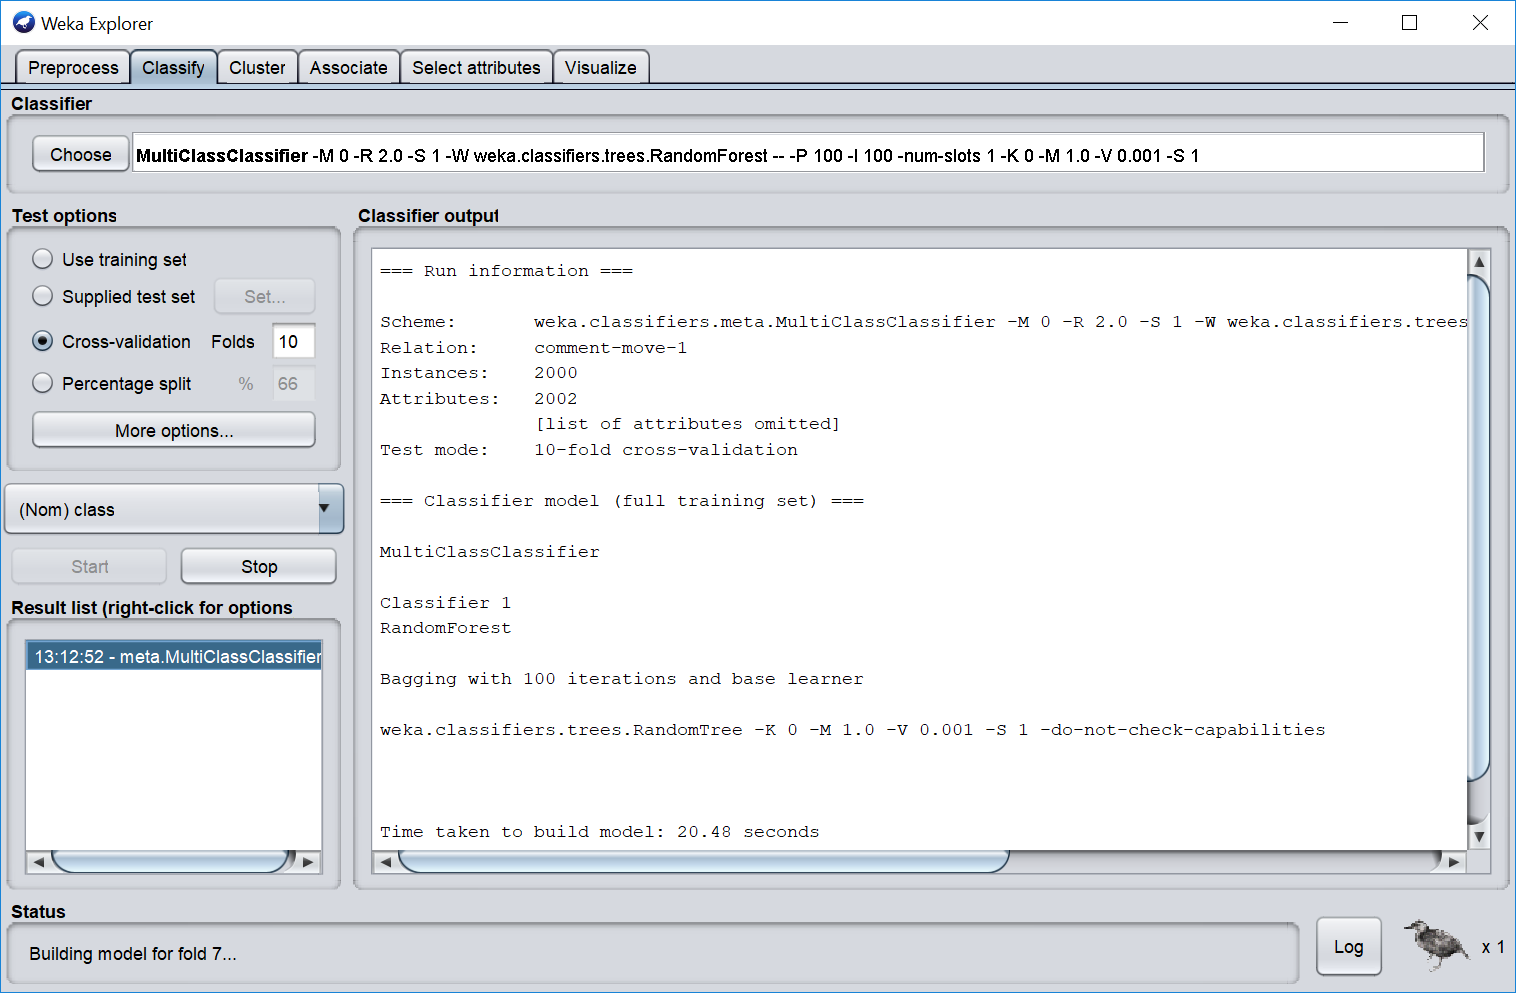
\includegraphics[scale=0.3]{images/weka_classify}
      \caption{Classification in Weka}
      \label{fig:weka_classify}
	\end{figure}
	
    Before the classification can be started, the data record must first be loaded from the ARFF file in the "Preprocess" tab. Finally, a suitable classifier for the problem can be selected via the "Choose" button and applied via "Start". The following classifiers - among others based on the algorithms described in sections~\ref{subsec:multiclass_classification}~and~\ref{subsec:multiclass_classification} - are used for the analysis:
    \begin{itemize}
      \item NaiveBayes (NB)

        The Naïve Bayes classifier uses a simple probabilistic model to predict the class of an instance. Since it calculates a probability value for each class, the classifier is also capable to handle multiclass problems. The classifier provides rather poor evaluation values, but is very fast and serves as a basic assessment of the problem and the models.
      \item RandomForest (RF)

        Random forests belong to the decision tree algorithms and use the ensemble learning method of bagging. The name random forest comes from the fact that a decision tree is created based on random subsets of the attributes. Thus, a forest of decision trees is formed, whereby the final prediction is made by equal weighting of all predictions of the trees. The training of the trees is fast and can be parallelized easily. Furthermore, the independence of the trained trees provides a robust model and good accuracy values. Random forests with 100 trees are used for testing. \\
For the following algorithms of the multiclass, ordinal class and nested dichotomy classifier, the random forest classifier will be used to solve the binary classification problems into which the multiclass problem is broken down.
      \item MultiClassClassifier, method 0 (MCC0)

        The multiclass classifier of Weka offers four different methods to break the multiclass classification problem down to multiple binary classification problems. The standard method with the ID 0 is the one-against-all approach.
      \item MultiClassClassifier, method 1 (MCC1)

        The algorithms using error-correcting output codes are as well included in the multiclass classifier. The method with ID 1 provides the ensemble learning with a random error-correcting output code.
      \item MultiClassClassifier, method 2 (MCC2)

        The method with ID 2 provides the ensemble learning with the exhaustive error-correcting output code. The code is therefore longer than the random code and needs more computing time.
      \item MultiClassClassifier, method 3 (MCC3)

        The last method with ID 3 is the one-against-one approach.
      \item MultiClassClassifier, method 3 with pairwise coupling (MCC3P)

        For the one-against-one approach, Weka additional offers the possibility to execute this algorithm with pairwise coupling.
      \item OrdinalClassClassifier (OCC)

        The ordinal class classifier can be installed separately and is based on the already introduced method of \citeauthor{Frank2001}, which divides a multiclass classification problem into binary classification problems considering the ordinal order of the class attribute. Of the classifiers tested, it is the only one to include this order in the classification process.
      \item ClassBalancedND (NDC)

        As for the ordinal class classifier, a package with nested dichotomy classifiers can be included as well. The class balanced nested dichotomy ensures a class equilibrium between the two subsets for each dichotomy.
      \item DataNearBalancedND (NDD)

        The other variant is the data near balanced nested dichotomy, where a data equilibrium between the two subsets for each dichotomy is ensured.
      \item ZeroR

        Finally, the zero-rule classifier is executed to provide a baseline that serves as comparison value for kappa statistics. The accuracy equals the percentage of the most frequent class and is therefore the same for all four models if the same data set is used.
    \end{itemize}
    Independent of the classifier, due to the higher number of attributes, the time required for the classification of the pre-trained word embedding model is about twice as long as for the own trained word embedding model and even five times as long for the count-based and TF-IDF-based models. Another factor for the computing time is the number of classes. However, additional classes also increase the required computing capacity. \\\\
    For the three multiclass classification problems, i.e. the move annotation problem with six classes and both position annotation problems, all classifiers can be applied to and provide different classification models and results. The two binary classification problems do not require any additional decomposition of the problem, so all multiclass classifiers and the ordinal class classifier output the same result as the underlying binary classification algorithm, in this case random forest. Thus, only Naïve Bayes, random forest and nested dichotomy remain for the binary classification problems as methods to be compared. \\\\
    The output of a classifier is the computed classification model, the correct and predicted classes for all instances if desired, and a set of evaluation metrics that will be discussed in the following chapter.

  \subsection{Evaluation Methods}    
  \label{subsec:evaluation_methods}
    The examined data sets have a size of 4,000 instances for the move vs. position annotation problem and a size of 2,000 instances for the other problems. The validation of the classification models is performed by 10-fold-cross-validation, i.e. 400 or 200 instances are hold out in each of the ten runs. All evaluation measurements will be averaged over the ten folds of the cross-validation. \\\\
    The main evaluation metric will be the accuracy. The higher the accuracy of a classification model, the better the classifier and the underlying feature model are evaluated. In order to be able to compare the accuracy across the different problems, the kappa statistic is used. The baseline determined by the zero-rule classifier is used as reference value for the calculation. \\\\
    In the configurations with the best accuracy, the confusion matrix is also analyzed. For all defined problems, the general occurrence probability of a class can influence the frequency of different misclassification types, i.e. the values $M_{ij}$ of the cells in the confusion matrix. However, this preference for frequent classes is not punished, since in all problems it is the same if $n$ instances of class $i$ are classified correctly or $n$ instances of class $j$. Besides, it does not matter if a class $i$ is misclassified as class $j$ or the misclassification happens the other way around. Under these circumstances, evaluation methods such as precision, recall and ROC are unsuitable. \\\\
However, the two above-mentioned conditions can be represented by a cost-sensitive evaluation matrix in which the entries of the main diagonal have the same cost, namely zero, and which is symmetrical, i.e. $c_{ij}=c_{ji}$. By this definition, the additional analysis by cost matrices for the two binary classification problems move vs. position annotations and good vs. poor moves is superfluous, the costs result automatically from the product of the misclassified instances with the only cost value different from zero. For the remaining three problems, both the total costs based on absolute and on squared cost vectors as presented in section~\ref{subsec:cost_sensitive_learning} are considered. An inclusion of these cost matrices in the classification process via cost-sensitive learning is not carried out.
  \clearpage  
  
  \section{Evaluation of Results}
  \label{sec:evaluation_of_results}
    In this chapter the results of the whole text mining process are presented and evaluated. The chapter starts with the test results of different tokenizer configurations. Then, based on the best tokenizer configuration, evaluations of the tokens in the chess annotation data are presented. Before applying the classifiers on the data sets, the feature models are evaluated separately by checking the most informative attributes and by applying basic queries on the word embeddings. Afterwards, the achieved accuracies for all combinations of problem, data set, model and classifier are compared and analyzed. Finally, the misclassifications are viewed using examples, confusion matrices and different cost weights.
      
  \subsection{Tokenizer Evaluation}    
  \label{subsec:tokenizer_evaluation}
    For the evaluation of the Tokenizer configurations, a small test set with a total of slightly more than 2,000 instances is used, which, however, includes all tokens, bigrams and trigrams that occur at least two times in the data set. Thus, the model contains nearly 13,000 attributes and is based on the counts of the terms. The Naïve Bayes classifier was used for the classification, which can consider all attributes without much additional calculation effort. As a further comparison value, the one-against-all classifier (MCC0) with random forest was used. In addition to the move annotation problems (too high computational effort), an attribute selection based on the gain ratio has been applied beforehand. In table~\ref{tab:tokenizer_statistics} the different tokenizer configurations and the percentage variance of their achieved accuracy in comparison to the one of the standard configuration are listed. Hence, improvements compared to the standard configuration are indicated by a "+".
    
	\begin{table}[H]
      \begin{tabular}{| l | r | r | r | r | r |}
    	\hline
    	Tokenizer & Total & Move-1 & Move-2 & Position-1 & Position-2 \\ \hline
	    \multirow{2}{*}{complete} & $86.0849\%$ & $76.6486\%$ & $54.3243\%$ & $43.4959\%$ & $21.9512\%$ \\	
	    & $86.5566\%$ & $75.6757\%$ & $55.3514\%$ & $51.2195\%$ & $19.9187\%$ \\ \hline
	    \multirow{2}{*}{no PGN non-standard codes} & $\pm0\%$ & $-0.07\%$ & $\pm0\%$ & $\pm0\%$ & $\pm0\%$ \\	
	    & $\pm0\%$ & $+0.50\%$ & $-0.68\%$ & $\pm0\%$ & $\pm0\%$ \\ \hline
	    \multirow{2}{*}{no NAG non-standard codes} & $\pm0\%$ & $\pm0\%$ & $\pm0\%$ & $\pm0\%$ & $\pm0\%$ \\	
	    & $+0.11\%$ & $+0.29\%$ & $-0.68\%$ & $\pm0\%$ & $\pm0\%$ \\ \hline
	    \multirow{2}{*}{no move-annotating symbols} & $\pm0\%$ & $\pm0\%$ & $-0.10\%$ & $-0.93\%$ & $\pm0\%$ \\	
	    & $\pm0\%$ & $+0.29\%$ & $-0.59\%$ & $\pm0\%$ & $\pm0\%$ \\ \hline
	    \multirow{2}{*}{no position-annotating symbols} & $\pm0\%$ & $-0.07\%$ & $-0.10\%$ & $\pm0\%$ & $\pm0\%$ \\	
	    & $+0.05\%$ & $-0.57\%$ & $-0.20\%$ & $\pm0\%$ & $\pm0\%$ \\ \hline
	    \multirow{2}{*}{no remis symbol} & $\pm0\%$ & $\pm0\%$ & $\pm0\%$ & $\pm0\%$ & $\pm0\%$ \\	
	    & $\pm0\%$ & $\pm0\%$ & $\pm0\%$ & $\pm0\%$ & $\pm0\%$ \\ \hline
	    \multirow{2}{*}{no abbreviations} & $+0.02\%$ & $-0.14\%$ & $-0.20\%$ & $+4.34\%$ & $-1.20\%$ \\	
	    & $-0.09\%$ & $-0.57\%$ & $-0.10\%$ & $-0.42\%$ & $-17.33\%$ \\ \hline
	    \multirow{2}{*}{no multiple dots} & $-0.16\%$ & $+0.07\%$ & $+0.30\%$ & $\pm0\%$ & $\pm0\%$ \\	
	    & $-1.42\%$ & $+0.29\%$ & $-0.59\%$ & $\pm0\%$ & $\pm0\%$ \\ \hline
	    \multirow{2}{*}{no merged words} & $-0.21\%$ & $-1.57\%$ & $+1.09\%$ & $+2.49\%$ & $-1.20\%$ \\	
	    & $+0.39\%$ & $-0.66\%$ & $-0.30\%$ & $+1.15\%$ & $-5.24\%$ \\ \hline
	    \multirow{2}{*}{no words} & $-0.51\%$ & $-4.79\%$ & $-10.92\%$ & $+2.79\%$ & $+8.23\%$ \\	
	    & $-1.01\%$ & $-2.99\%$ & $-1.56\%$ & $-12.71\%$ & $+23.61\%$ \\ \hline
	    \multirow{2}{*}{no remaining non-whitespace characters} & $-0.27\%$ & $-0.56\%$ & $-0.50\%$ & $-3.74\%$ & $-11.11\%$ \\	
	    & $+0.33\%$ & $-0.21\%$ & $-1.07\%$ & $\pm0\%$ & $\pm0\%$ \\ \hline
      \end{tabular}
      \caption{Accuracies for different RegexTokenizer}
      \label{tab:tokenizer_statistics}
	\end{table}

    The removal of the regular expressions for PGN or NAG non-standard codes as well as the removal of those for move- or position-annotating symbols had a slight deterioration of the accuracy as a consequence while the removal of the remis symbol as a token had no effect at all. The removal of the regular expression for abbreviations which also matches move counts, had a negative influence on the accuracy in eight of ten cases. For the regular expression for multiple dots, there were three improvements and three deteriorations, with the deteriorations weighing heavier. In the last three regular expressions for merged words, words and remaining non-whitespace characters, more than half of the accuracy values deteriorated. There are noticeable improvements for the position annotation problem with seven classes by the exclusion of words, i.e. the positions could be determined better by the counts of the letters than by the counts of the words. At the same time, however, this adaptation also led to significant deteriorations in the other problems. Overall, for all comparison configurations, the sum of the degradations is at least as large as the sum of the improvements, which is why the initial configuration of the tokenizer is retained. \\\\
    The tokenizer tests were executed before the additional chess files of the Mega Database 2012 were available. For this reason, the ChessBase data sets were not included, which results in a different class distribution, especially in the move vs. position annotation problem. The high values of over 85\% accuracy in the first column can be explained by the fact that in this first test data set about seven eighths of the comments were move annotations. Thus, the baseline is even above the best accuracy. In order to have absolute certainty that the best tokenizer configuration in the tests will also perform best for the new datasets, the datasets would have to be recreated and re-tested.
 
  \subsection{Data Set Evaluation}    
    After the determination of the tokenizer, the used comment data can be processed uniformly into tokens. For a better understanding of the data, some statistics regarding those tokens are created. In the evaluations in this section, the tokens were converted to lowercase, but not lemmatized. Filtering by language or minimum comment length was also not performed. \\\\
    In the first step, the number of comments is analyzed depending on their length in tokens. The statistics are shown in table~\ref{tab:comment_length} and figure~\ref{fig:comment_length}. It can be seen that about half of the comments have a maximum token count of nine. 99 of these comments do not even contain a single token, since they consist only of whitespace characters. Of the remaining comments, only a small portion has a length of at least 50 tokens. Due to these circumstances, a length of three to nine tokens was defined for short comments and a length of ten to 49 tokens for long comments.

    \begin{figure}[H]
      \begin{floatrow}
      \capbtabbox[7cm]{%
	  \begin{tabular}{ | c | r | }
		\hline
		Length & Count \\ \hline
		0-4 & 92,519 \\ \hline
		5-9 & 154,412 \\ \hline
		10-14 & 105,778 \\ \hline
		15-19 & 77,983 \\ \hline
		20-29 & 52,802 \\ \hline
		30-49 & 21,480 \\ \hline
		50-99 & 5,653 \\ \hline
		100-199 & 586 \\ \hline
		200+ & 60 \\ \hline
		\hline
		all & 511,273 \\ \hline
	  \end{tabular}
      }{%
        \caption{Comment length in tokens}
        \label{tab:comment_length}
      }
      \ffigbox[10cm]{%
	    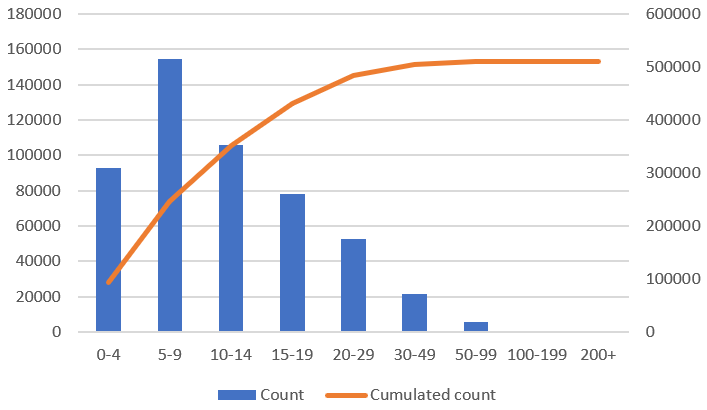
\includegraphics[scale=0.75]{images/comment_length}
      }{%
	    \caption{Count and cumulative count of comment length}
        \label{fig:comment_length}
      }
      \end{floatrow}
    \end{figure}

    Likewise, statistics about the tokens themselves can be created. An evaluation of how many tokens, bigrams and trigrams exist with a certain number of minimum occurrences is relevant because it determines the maximum number of attributes for the count- and TF-IDF-based model. This number is given for different numbers of at minimum occurrences in table~\ref{tab:frequency_tokens_bigrams_trigrams}. It should be noted that this number will be smaller if a lemmatization is applied beforehand.
    
	\begin{table}[H]
	  \begin{tabular}{ | r | r | r | r | }
		\hline
		Min. occurrences & Count tokens & Count bigrams & Count trigrams \\ \hline
		1,000 & 654 & 458 & 130 \\ \hline
		300 & 1,719 & 1,948 & 706 \\ \hline
		100 & 3,913 & 6,382 & 3,013 \\ \hline
		30 & 9,280 & 21,730 & 15,314 \\ \hline
		10 & 20,881 & 63,250 & 60,923 \\ \hline
		3 & 51,693 & 204,975 & 286,032 \\ \hline
		1 & 158,652 & 798,608 & 1,869,193 \\ \hline
	  \end{tabular}
      \caption{Frequency of tokens, bigrams and trigrams}
      \label{tab:frequency_tokens_bigrams_trigrams}
	\end{table}
	
    Due to the many possible combinations, there is a very large total number of trigrams, which, however, decreases rapidly when the threshold is increased. In the case of bigrams, this tendency is not so pronounced. Even for a threshold value of 300 there are more bigrams than single tokens. Altogether it can be stated that a threshold of three already reduces the number of possible attributes to about 20\% and a threshold of ten even to 5\% of the original number. From the top row we can conclude that there are only slightly more than 1,000 terms which occur in at least 0.2\% of the comments. This indicates a strong variance in the comments. \\\\
    Besides, additional analyses were performed to determine the most common words, bigrams and trigrams. The values can be seen in the tables~\ref{tab:frequent_tokens},~\ref{tab:frequent_bigrams}~and~\ref{tab:frequent_trigrams}. It is not sure whether such frequently occurring terms are meaningful at all, i.e. whether they offer an information gain. If this is the case, however, they can be used very well as learning and decision criteria, because they can be applied to a large number of comments.
          
	\begin{table}[H]
      \subfloat[all tokens]{
      \begin{tabular}{| l | r |}
    	\hline
		Token & Count \\ \hline
	    , & 459,014 \\ \hline
	    / & 310,510 \\ \hline
		. & 241,009 \\ \hline
		the & 138,730 \\ \hline
		[ & 123,708 \\ \hline
		] & 123,670 \\ \hline
		) & 116,210 \\ \hline
		( & 115,868 \\ \hline
		\% & 111,512 \\ \hline
		a & 70,800 \\ \hline
      \end{tabular}
      }
      \quad
      \quad
      \quad
      \subfloat[all English words]{
      \begin{tabular}{ | l | r | }
		\hline
		Token & Count \\ \hline
		the & 138,730 \\ \hline
		a & 70,800 \\ \hline
		to & 64,120 \\ \hline
		cal & 60,054 \\ \hline
		is & 56,347 \\ \hline
		black & 42,819 \\ \hline
		white & 41,679 \\ \hline
		in & 39,794 \\ \hline
		and & 38,725 \\ \hline
		of & 36,566 \\ \hline
	  \end{tabular}
      }
      \quad
      \quad
      \quad
      \subfloat[all English non-stopwords]{
      \begin{tabular}{ | l | r | }
		\hline
		Token & Count \\ \hline
		cal & 60,054 \\ \hline
		black & 42,819 \\ \hline
		white & 41,679 \\ \hline
		move & 22,431 \\ \hline
		die & 18,428 \\ \hline
		position & 16,599 \\ \hline
		schwarz & 14,037 \\ \hline
		v & 13,798 \\ \hline
		ist & 12,849 \\ \hline
		game & 12,178 \\ \hline
	  \end{tabular}
      }
      \caption{Most frequent tokens in comments}
      \label{tab:frequent_tokens}
	\end{table}
	
    Among the most common tokens, bigrams and trigrams are mainly punctuation marks and combinations of those that do not allow intuitive conclusions to be made about certain annotation types. The only exceptions are the bigrams "1/2 -" and "- 1/2" respectively the trigram "1/2 - 1/2", which could indicate a balanced position. If the list is limited to English words, there are numerous stopwords and combinations of these, but also the two tokens "white" and "black" and the phrases "this move", "the game" or "week in chess". If you consider only non-stopwords for the tokens, then with the words "move" and "position" two further interesting tokens are among the top ten, which should be relevant at least for the classification according to move and position annotations.
    
    \begin{figure}[H]
      \begin{floatrow}
      \capbtabbox[8.5cm]{%
      \subfloat[all bigrams]{
      \begin{tabular}{| l | r |}
    	\hline
		Bigram & Count \\ \hline
		[ \% & 111,424 \\ \hline
		\% cal & 60,054 \\ \hline
		\% csl & 51,190 \\ \hline
		/ \textbackslash & 26,923 \\ \hline
		1/2 - & 19,115 \\ \hline
		, a & 18,829 \\ \hline
		- 1/2 & 18,605 \\ \hline
		] [ & 18,169 \\ \hline
		/ cbm & 15,877 \\ \hline
		) / & 14,837 \\ \hline
      \end{tabular}
      }
      \quad
      \subfloat[all English bigrams]{
      \begin{tabular}{ | l | r | }
		\hline
		Bigram & Count \\ \hline
		of the & 10,650 \\ \hline
		on the & 10,381 \\ \hline
		in the & 9,779 \\ \hline
		the game & 7,464 \\ \hline
		this move & 6,667 \\ \hline
		white has & 5,829 \\ \hline
		black has & 5,711 \\ \hline
		for the & 5,650 \\ \hline
		this is & 5,090 \\ \hline
		to the & 4,613 \\ \hline
	  \end{tabular}
      }
      }{%
        \caption{Most frequent bigrams in comments}
        \label{tab:frequent_bigrams}
      }
      \capbtabbox[8.5cm]{%
      \subfloat[all trigrams]{
      \begin{tabular}{| l | r |}
    	\hline
		Trigram & Count \\ \hline
		[ \% cal & 60,054 \\ \hline
		[ \% csl & 51,190 \\ \hline
		1/2 - 1/2 & 18,603 \\ \hline
		] [ \% & 17,863 \\ \hline
		, a / & 13,696 \\ \hline
		, v / & 9,252 \\ \hline
		, m / & 8,728 \\ \hline
		, j / & 8,717 \\ \hline
		, s / & 6,229 \\ \hline
		, r / & 5,096 \\ \hline
      \end{tabular}
      }
      \quad
      \subfloat[all English trigrams]{
      \begin{tabular}{ | l | r | }
		\hline
		Trigram & Count \\ \hline
		week in chess & 2,322 \\ \hline
		the week in & 2,319 \\ \hline
		this is the & 1,651 \\ \hline
		in the game & 1,566 \\ \hline
		this move is & 1,498 \\ \hline
		in order to & 1,217 \\ \hline
		white has a & 1,203 \\ \hline
		this is a & 1,117 \\ \hline
		of the game & 1,018 \\ \hline
		in view of & 968 \\ \hline
	  \end{tabular}
      }
      }{%
        \caption{Most frequent trigrams in comments}
        \label{tab:frequent_trigrams}
      }
      \end{floatrow}
	\end{figure}

  \subsection{Model Evaluation}    
    Before the classification is performed, some analyses can already be done on the underlying models. In the two models, where each attribute correlates with a certain term, namely the count-based model and the TF-IDF-based model, meaningful attributes and thus terms that are relevant for classification decisions can be determined by calculating values such as the gain ratio. Table~\ref{tab:most_informative_attributes} shows the ten best attributes by gain ratio for the move vs. position annotation problem, the move annotation problem with two classes and the position annotation problem with three classes. In the following, no distinction is made between the count-based model and the TF-IDF-based model, since the values are very similar in both models. \\\\
    The best attributes for the move annotation problem all indicate a poor move and are intuitive or at least comprehensible like count(be too). The position annotation problem also includes three intuitively useful attributes: count(white loose), count(balance) and count(equalize). For the rest, it is not obvious at first glance to what extent the classes are differentiated by the attribute. Even less obvious are the statements of the best rated attributes (except the last one) of the move vs. position annotation problem. Though, here the gain ratio values are generally lower.
    
	\begin{table}[H]
      \subfloat[Move vs. position]{
      \begin{tabular}{| l | r |}
    	\hline
		Feature & Gain \\ \hline
		count(the week in) & 0.14348 \\ \hline
		count(the week) & 0.14348 \\ \hline
		count(week) & 0.14348 \\ \hline
		count(week in) & 0.14348 \\ \hline
		count(week in chess) & 0.14348 \\ \hline
		count(in chess) & 0.14348 \\ \hline
		count(/ the week) & 0.14348 \\ \hline
		count(/) & 0.14107 \\ \hline
		count(ext) & 0.13853 \\ \hline
		count(1/2) & 0.13752 \\ \hline
      \end{tabular}
      }
      \subfloat[Move (2 classes)]{
      \begin{tabular}{ | l | r | }
		\hline
		Feature & Gain \\ \hline
		count(mistake) & 0.21430 \\ \hline
		count(blunder) & 0.20024 \\ \hline
		count(decisive mistake) & 0.18957 \\ \hline
		count(decisive mistake .) & 0.18122 \\ \hline
		count(be too) & 0.17391 \\ \hline
		count(mistake .) & 0.17252 \\ \hline
		count(mistake ,) & 0.17119 \\ \hline
		count(the decisive mistake) & 0.16829 \\ \hline
		count(blunder .) & 0.16829 \\ \hline
		count(time trouble) & 0.16177 \\ \hline
	  \end{tabular}
      }
      \subfloat[Position (3 classes)]{
      \begin{tabular}{ | l | r | }
		\hline
		Feature & Gain \\ \hline
		count(white lose) & 0.23008 \\ \hline 
		count(the text) & 0.21687 \\ \hline 
		count(balance) & 0.21345 \\ \hline
		count(equalize) & 0.21345 \\ \hline
		count(repetition) & 0.21345 \\ \hline
		count(win a pawn) & 0.20842 \\ \hline
		count(play for a) & 0.20842 \\ \hline
		count(queen .) & 0.20842 \\ \hline
		count(ha no problem) & 0.20776 \\ \hline
		count(no problem) & 0.20776 \\ \hline
	  \end{tabular}
      }
      \caption{Most informative attributes in comments}
      \label{tab:most_informative_attributes}
	\end{table}
	
    The attributes shown in table~\ref{tab:most_informative_attributes}, however, show partly strong dependencies to each other. If the attribute count(mistake) is already selected in the case of the move annotation problem, the attributes count(mistake .) and count(mistake ,) are redundant and no longer provide any additional information gain. For this reason, the rule-based classifier J48 was used to create a classification model with rules for the three problems mentioned in order to investigate suitable attribute combinations. The learned rules are structured according to the scheme "(condition A) and (condition B) => prediction (true positive count, false positive count) and can be seen in figure~\ref{fig:move_rules},~\ref{fig:position_rules}~and~\ref{fig:move_vs_position_rules}. Note that in each case the last rule has no condition and predicts the most frequent class.
        
	\begin{figure}[H]
	  \centering
	  \begin{lstlisting}	  
(count(mistake) >= 1) => class=2 (65.0/2.0)
(number_of_tokens <= 5) and (count(.) <= 0) and (count(of) >= 1) => class=2 (17.0/2.0)
(count(but) >= 1) and (count(this) >= 1) and (count(of) <= 0) => class=2 (49.0/16.0)
(count(lose) >= 1) and (number_of_tokens <= 13) => class=2 (37.0/7.0)
(number_of_tokens <= 5) and (count(by) >= 1) => class=2 (17.0/1.0)
(count(miss) >= 1) and (count(miss_this) <= 0) => class=2 (30.0/4.0)
(count(wa) >= 1) and (number_of_tokens >= 10) and (count(_comma_) <= 0) 
	=> class=2 (48.0/15.0)
(count(blunder) >= 1) => class=2 (21.0/0.0)
(number_of_tokens <= 6) and (count(too) >= 1) => class=2 (9.0/0.0)
(count(allow) >= 1) => class=2 (35.0/10.0)

 => class=1 (1672.0/413.0)
	  \end{lstlisting}
      \caption{Rules for the 2-class move annotation problem}
      \label{fig:move_rules}
	\end{figure}
	
	\begin{figure}[H]
	  \centering
	  \begin{lstlisting}	  
(count(0-1) >= 1) and (number_of_tokens >= 18) => class=3 (58.0/26.0)
(count(/) <= 0) and (count(win) >= 1) and (count(white) <= 0) and 
	(number_of_tokens >= 9) => class=3 (34.0/11.0)
	
(count(1/2) >= 1) and (count(ext) <= 0) => class=2 (136.0/65.0)

 => class=1 (1772.0/733.0)
	  \end{lstlisting}
      \caption{Rules for the 3-class position annotation problem}
      \label{fig:position_rules}
	\end{figure}
	
    As in the tables, the rules for the move and position annotation problem are largely comprehensible, whether intuitive or not. In addition, the comment length seems to be relevant as it is used as part of rules in both models. The rules of the move vs. position annotation problem, on the other hand, are less comprehensible and it is questionable whether they could also be successfully applied in other data sets.
    	
	\begin{figure}[H]
	  \centering
	  \begin{lstlisting}	  
(count(/) >= 1) and (count(/_\) <= 0) => class=2 (699.0/49.0)
(count(and) >= 1) and (number_of_tokens <= 19) and (count(white) >= 1) 
	=> class=2 (153.0/35.0)
(count(to) <= 0) and (count(and) >= 1) and (count(ha) >= 1) => class=2 (71.0/12.0)
(count(this) <= 0) and (count(to) <= 0) and (count(.) >= 1) and (count(the) <= 0) and 
	(count(with) >= 1) => class=2 (97.0/16.0)
(count(move) <= 0) and (count(be) >= 1) and (count(the) <= 1) and (count(.) >= 1) and 
	(count(this) <= 0) => class=2 (504.0/194.0)
(count(move) <= 0) and (count(_comma_) >= 2) and (count(to) <= 0) 
	=> class=2 (117.0/45.0)
(count(move) <= 0) and (count(ha) >= 1) and (count(to) <= 0) => class=2 (85.0/32.0)

 => class=1 (2274.0/657.0)
	  \end{lstlisting}
      \caption{Rules for the move vs. position annotation problem}
      \label{fig:move_vs_position_rules}
	\end{figure}
	
    For the word embeddings an evaluation like for the count- and TF-IDF-based models is not useful, because the concrete statements by the attributes of the word embeddings are unknown. Instead, the learned vectors of the vocabulary can be compared directly with each other to check whether the semantics of the comments have been captured meaningfully. For this purpose, the most similar words to the (chess) terms "check" and "blunder" with respect to the cosine similarity are compared for the word embedding learned on the chess comments (see table~\ref{tab:cosine_similarities_w2v_own}) and the word embedding learned on Google News (see table~\ref{tab:cosine_similarities_w2v_pretrained}).

    \begin{figure}[H]
      \begin{floatrow}
      \capbtabbox[8.1cm]{%
      \subfloat[Most similar to "check"]{
      \begin{tabular}{| l | r |}
		\hline
		Word & Similarity \\ \hline
		mate & 0.5111 \\ \hline
		pin & 0.5075 \\ \hline
		capture & 0.4505 \\ \hline
		fork & 0.4442 \\ \hline
		move & 0.4145 \\ \hline
		perpetual & 0.4108 \\ \hline
		guard & 0.3812 \\ \hline
		penetration & 0.3736 \\ \hline
		threat & 0.3591 \\ \hline
		attack & 0.3498 \\ \hline
      \end{tabular}
      }
      \quad
      \subfloat[Most similar to "blunder"]{
      \begin{tabular}{ | l | r | }
		\hline
		Word & Similarity \\ \hline
		mistake & 0.8191 \\ \hline
		error & 0.7349 \\ \hline
		oversight & 0.7288 \\ \hline
		miscalculation & 0.6497 \\ \hline
		inaccuracy & 0.6169 \\ \hline
		touch & 0.5317 \\ \hline
		time-trouble & 0.5077 \\ \hline
		blow & 0.4959 \\ \hline
		shoot & 0.4909 \\ \hline
		concession & 0.4849 \\ \hline
	  \end{tabular}
      }
      }{%
        \caption{Cosine similarities in chess word2vec-model}
        \label{tab:cosine_similarities_w2v_own}
      }
      \capbtabbox[8.9cm]{%
      \subfloat[Most similar to "check"]{
      \begin{tabular}{| l | r |}
		\hline
		Word & Similarity \\ \hline
		checking & 0.7029 \\ \hline
		checks & 0.6817 \\ \hline
		checked & 0.6749 \\ \hline
		Checking & 0.5686 \\ \hline
		recheck & 0.5329 \\ \hline
		doublecheck & 0.5239 \\ \hline
		Check & 0.5161 \\ \hline
		VGGEN\_often & 0.5077 \\ \hline
		Charge\_Issuing\_worthless & 0.4998 \\ \hline
		ABCActionNews.com & 0.4760 \\ \hline
      \end{tabular}
      }
      \quad
      \subfloat[Most similar to "blunder"]{
      \begin{tabular}{ | l | r | }
		\hline
		Word & Similarity \\ \hline
		gaffe & 0.7873 \\ \hline
		blunders & 0.7614 \\ \hline
		mistake & 0.7505 \\ \hline
		faux\_pas & 0.6696 \\ \hline
		miscue & 0.6602 \\ \hline
		misjudgment & 0.6521 \\ \hline
		howler & 0.6513 \\ \hline
		bungle & 0.6400 \\ \hline
		tactical\_blunder & 0.6219 \\ \hline
		miscalculation & 0.6167 \\ \hline
	  \end{tabular}
      }
      }{%
        \caption{Cosine similarities in Google News word2vec-model}
        \label{tab:cosine_similarities_w2v_pretrained}
      }
      \end{floatrow}
	\end{figure}

    The self-trained word embedding gives as expected a list of related chess terms, while the pretrained word embedding calculates more general terms, which should be irrelevant for the chess comments. For the two words "mistake" and "miscalculation", which occur in both tables, the self-trained word embedding has higher similarity values to the given word "blunder" than the pretrained word embedding. Furthermore, the self-trained word embedding achieves a similarity of 97.78\% for the two words "white" and "black", whereas in the pretrained word embedding it is only 80.92\%. In principle, a similarity of these terms is desired, but a similarity that is too high could make it difficult to distinguish the two words from each other and thus complicate decisions whether a position is in favor of white or in favor of black.
    
  \subsection{Classification Results}
    In this thesis five different problems, four different models, ten different classifiers and three different data sets were presented. For all meaningful combinations of these variables, a classification was performed and the accuracy calculated. This section summarizes these results. All accuracies of the first data set are displayed and analyzed in tabular and graphical form for each problem. The best values are then compared with those of the two remaining data sets. \\\\
    In all tables the classifiers have the abbreviations as described in section~\ref{subsec:classification_algorithms}, furthermore the word embeddings are abbreviated with w2v-C for the model learned on the chess comments and w2v-GN for the model learned on Google News. The highest value of each table is marked in bold. In the case of the multiclass classification problems, the accuracies of the two error-correcting output code classifiers (MCC1 \& MCC2) were not determined due to excessive computation time. Therefore, these two classifiers, as well as the Naïve Bayes classifier, whose values fell sharply compared to the rest, are not shown in the diagrams.

    \begin{figure}[H]
      \begin{floatrow}
      \capbtabbox[8.5cm]{%
	  \begin{tabular}{ | l | r | r | r | r | }
		\hline
		   & count  & TF-IDF & w2v-C  & w2v-GN  \\ \hline
		ND & 0.7785 & 0.7725 & 0.7345 & 0.7258  \\ \hline
		RF & \textbf{0.7825} & 0.7728 & 0.7368 & 0.7180  \\ \hline
		NB & 0.6963 & 0.7030 & 0.6630 & 0.6265  \\ \hline
		Baseline & \multicolumn{4}{c|}{0.5000} \\ \hline
	  \end{tabular}
       }{%
        \caption{Accuracies for move vs. position annotation problem}
        \label{tab:total}
      }
      \ffigbox[8.5cm]{%
	    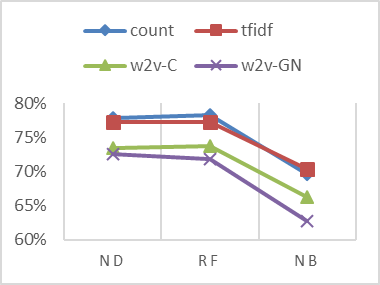
\includegraphics{images/total}
      }{%
	    \caption{Comparison of accuracies for move vs. position annotation problem}
        \label{fig:total}
      }
      \end{floatrow}
    \end{figure}

On the move vs. position annotations only the classifiers random forest, nested dichotomy and Naïve Bayes are applied because it is a binary classification problem. As seen in table~\ref{tab:total} and figure~\ref{fig:total}, a maximum accuracy of 78.25\% is achieved with the count-based model and the random forest classifier. The same classifiers are also applied to the second binary classification problem of move annotations (see table~\ref{tab:move_1} and figure~\ref{fig:move_1}). This time, the classifier nested dichotomy reaches the best accuracy of 76.90\%, again using the count-based model.

    \begin{figure}[H]
      \begin{floatrow}
      \capbtabbox[8.5cm]{%
	  \begin{tabular}{ | l | r | r | r | r | }
		\hline
		   & count  & TF-IDF & w2v-C  & w2v-GN  \\ \hline
		ND & \textbf{0.7690} & 0.7575 & 0.6735 & 0.7305  \\ \hline
		RF & 0.7590 & 0.7610 & 0.6670 & 0.7335  \\ \hline
		NB & 0.6355 & 0.5990 & 0.4555 & 0.6895  \\ \hline
		Baseline & \multicolumn{4}{c|}{0.6580} \\ \hline
	  \end{tabular}
       }{%
        \caption{Accuracies for move annotation problem (2~classes)}
        \label{tab:move_1}
      }
      \ffigbox[8.5cm]{%
	    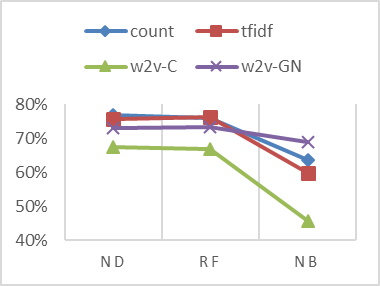
\includegraphics{images/move_1}
      }{%
	    \caption{Comparison of accuracies for move annotation problem (2~classes)}
        \label{fig:move_1}
      }
      \end{floatrow}
    \end{figure}

All ten classifiers are applied to the three multiclass classification problems. Table~\ref{tab:move_2} shows the results for the move annotation problem with six classes and a best value of 54.90\% for the count-based model and the one-against-all classifier. It can be seen in figure~\ref{fig:move_2} that for all classifiers the count-based model achieves the highest accuracies, closely followed by the TF-IDF model. The accuracies of the Google News word embeddings are about five percentage points below these models and the chess word embeddings even about ten percentage points below. This ranking of the models had already been indicated by the first two problems.

    \begin{figure}[H]
      \begin{floatrow}
      \capbtabbox[8.5cm]{%
	  \begin{tabular}{ | l | r | r | r | r | }
		\hline
		      & count  & TF-IDF & w2v-C  & w2v-GN \\ \hline
		MCC0  & \textbf{0.5490} & 0.5405 & 0.4445 & 0.4985 \\ \hline
		MCC3  & 0.5420 & 0.5265 & 0.4415 & 0.4930 \\ \hline
		MCC3P & 0.5425 & 0.5300 & 0.4470 & 0.4855 \\ \hline
		OCC   & 0.5475 & 0.5320 & 0.4360 & 0.4990 \\ \hline
		NDC   & 0.5445 & 0.5295 & 0.4465 & 0.4960 \\ \hline
		NDD   & 0.5435 & 0.5285 & 0.4525 & 0.4895 \\ \hline
		RF    & 0.5330 & 0.5285 & 0.4400 & 0.4920 \\ \hline
		NB    & 0.4025 & 0.1750 & 0.1945 & 0.2435 \\ \hline
		MCC1  & \multicolumn{2}{r|}{} & 0.4085 & 0.4790 \\ \hline
		MCC2  & \multicolumn{2}{r|}{} & 0.4550 & 0.4975 \\ \hline
		Baseline & \multicolumn{4}{c|}{0.4430}   \\ \hline
	  \end{tabular}
       }{%
        \caption{Accuracies for move annotation problem (6~classes)}
        \label{tab:move_2}
      }
      \ffigbox[8.5cm]{%
	    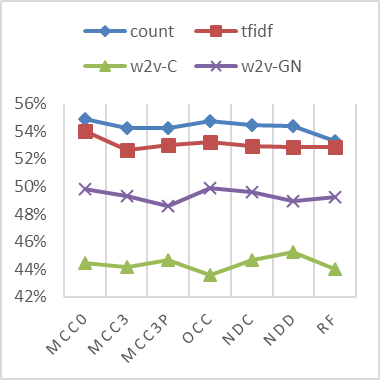
\includegraphics{images/move_2}
      }{%
	    \caption{Comparison of accuracies for move annotation problem (6~classes)}
        \label{fig:move_2}
      }
      \end{floatrow}
    \end{figure}

As well for the position annotation problem with three classes the count-based model proves to be the best (see table~\ref{tab:position_1} and figure~\ref{fig:position_1}). Again, the maximum value is achieved with another classifier, this time the one-against-one classifier with pairwise coupling. The accuracy value of 56.80\% is only slightly above the baseline, which corresponds to a kappa statistic of less than three percent. Previously, maximum kappa values of 56.5\% (move vs. position), 36.5\% (move, 2 classes) and 19\% (move, 6 classes) were reached. For the position annotation problem with seven classes the kappa value is again over 15\%. These values are therefore very low overall, although this is partly due to class imbalance.

    \begin{figure}[H]
      \begin{floatrow}
      \capbtabbox[8.5cm]{%
	  \begin{tabular}{ | l | r | r | r | r | }
		\hline
		      & count  & TF-IDF & w2v-C  & w2v-GN \\ \hline
		MCC0  & 0.5670 & 0.5570 & 0.5410 & 0.5645 \\ \hline
		MCC3  & 0.5620 & 0.5600 & 0.5410 & 0.5600 \\ \hline
		MCC3P & \textbf{0.5680} & 0.5620 & 0.5455 & 0.5620 \\ \hline
		OCC   & 0.5570 & 0.5560 & 0.5395 & 0.5645 \\ \hline
		NDC   & 0.5595 & 0.5520 & 0.5385 & 0.5615 \\ \hline
		NDD   & 0.5595 & 0.5560 & 0.5500 & 0.5615 \\ \hline
		RF    & 0.5600 & 0.5645 & 0.5445 & 0.5640 \\ \hline
		NB    & 0.4100 & 0.3545 & 0.2755 & 0.3080 \\ \hline
		MCC1  & \multicolumn{2}{r|}{} & 0.5300 & 0.5460 \\ \hline
		MCC2  & \multicolumn{2}{r|}{} & 0.5435 & 0.5660 \\ \hline
		Baseline & \multicolumn{4}{c|}{0.5550}   \\ \hline
	  \end{tabular}
       }{%
        \caption{Accuracies for position annotation problem (3~classes)}
        \label{tab:position_1}
      }
      \ffigbox[8.5cm]{%
	    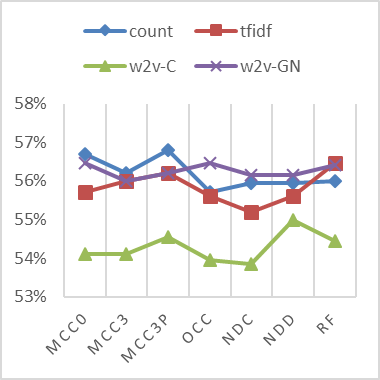
\includegraphics{images/position_1}
      }{%
	    \caption{Comparison of accuracies for position annotation problem (3~classes)}
        \label{fig:position_1}
      }
      \end{floatrow}
    \end{figure}

The lowest accuracies by far are achieved in the position annotation problem with seven classes (see table~\ref{tab:position_2} and figure~\ref{fig:position_2}). The maximum value of 36,20\% is reached in the count-based model by the one-against-one classifier with pairwise coupling as well as by the class balanced nested dichotomy classifier. Again the diagram shows the clear ranking of the models: count-based-model followed by TF-IDF-based model, Google News word embedding and chess word embedding.

    \begin{figure}[H]
      \begin{floatrow}
      \capbtabbox[8.5cm]{%
	  \begin{tabular}{ | l | r | r | r | r | }
		\hline
		      & count  & TF-IDF & w2v-C  & w2v-GN \\ \hline
		MCC0  & 0.3520 & 0.3490 & 0.2940 & 0.3100 \\ \hline
		MCC3  & 0.3565 & 0.3480 & 0.2905 & 0.3250 \\ \hline
		MCC3P & \textbf{0.3620} & 0.3525 & 0.2905 & 0.3360 \\ \hline
		OCC   & 0.3365 & 0.3420 & 0.2855 & 0.2980 \\ \hline
		NDC   & \textbf{0.3620} & 0.3340 & 0.2880 & 0.3160 \\ \hline
		NDD   & 0.3545 & 0.3420 & 0.2875 & 0.3205 \\ \hline
		RF    & 0.3425 & 0.3405 & 0.2790 & 0.2865 \\ \hline
		NB    & 0.2525 & 0.2190 & 0.1815 & 0.1930 \\ \hline
		MCC1  & \multicolumn{2}{r|}{} & 0.2620 & 0.2805 \\ \hline
		MCC2  & \multicolumn{2}{r|}{} & 0.2900 & 0.3295 \\ \hline
		Baseline & \multicolumn{4}{c|}{0.2465}   \\ \hline
	  \end{tabular}
       }{%
        \caption{Accuracies for position annotation problem (7~classes)}
        \label{tab:position_2}
      }
      \ffigbox[8.5cm]{%
	    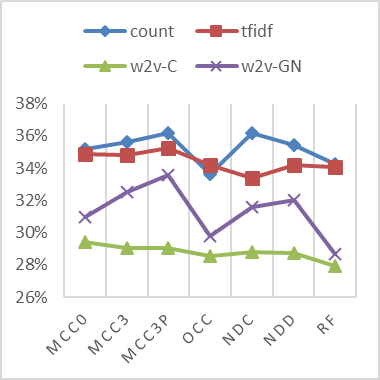
\includegraphics{images/position_2}
      }{%
	    \caption{Comparison of accuracies for position annotation problem (7~classes)}
        \label{fig:position_2}
      }
      \end{floatrow}
    \end{figure}

Overall, the results of the five tables and figures show that the count-based model is the best, followed by the TF-IDF-based model and the chess word embedding is the worst. Among the classifiers, there was no clear trend which is best. These observations are also confirmed by the other two data sets. The count-based model has the highest average accuracy holding 13 of the 15 best accuracy values (see table~\ref{tab:comparison_accuracies}). The other two best values are reached by the TF-IDF-based model, which is partially superior to the count-based model in the data set with long comments. The nested dichotomies classifiers achieve the best values overall, whereby the accuracies are only slightly above those of the other classifiers and therefore no conclusion can be drawn. \\\\
However, it is noticeable that the data set with the short comments achieves significantly better accuracies than the mixed-length data set. The only exception is the move vs. position annotation problem. The accuracies for the data set with long comments are on average slightly lower than for the mixed-length data set. These values suggest that either the short comments are generally more meaningful or that the condition that at least three English words must occur in the comment filters out qualitatively inferior short comments, while most qualitatively inferior long comments remain in the data set.

    \begin{table}[H]
      \subfloat[Accuracies]{
	  \begin{tabular}{ | l | r | r | r | r | r | }
		\hline
		Data set & Position vs. Move & Move (2 classes) & Move (6 classes) & Position (3 Classes) & Position (7 Classes) \\ \hline
		mixed & 0.7825 & 0.7690 & 0.5490 & 0.5680 & 0.3620 \\ \hline
		short & 0.7495 & 0.8134 & 0.5670 & 0.5985 & 0.4210 \\ \hline
		long  & 0.7813 & 0.7535 & 0.5275 & 0.5890 & 0.3535 \\ \hline
	  \end{tabular}
      }      
      \quad      
      \subfloat[Model + Classifier]{
	  \begin{tabular}{ | l | r | r | r | r | r | }
		\hline
		Data set & Position vs. Move & Move (2 classes) & Move (6 classes) & Position (3 Classes) & Position (7 Classes) \\ \hline
		mixed & Count + RF & Count + ND & Count + MCC0 & Count + MCC3P & Count + NDC/MCC3P \\ \hline
		short & Count + ND & Count + ND & Count + NDD & Count + RF & Count + NDC \\ \hline
		long & TF-IDF + ND & Count + ND & Count + MCC0 & TF-IDF + NDD & Count + NDD \\ \hline
	  \end{tabular}
      }
      \caption{Comparison of the best achieved accuracies}
      \label{tab:comparison_accuracies}
	\end{table}
  \clearpage

  \subsection{Misclassifications}
    The classification results obtained in the previous section have so far only been evaluated according to the accuracy value. In this section, the misclassifications are examined and it is checked whether the previously optimal results remain optimal even after weighting the misclassifications with costs. First, the confusion matrices are used to analyze which types of misclassifications frequently occur. The confusion matrices of the ordinal class classifier in table~\ref{tab:confusion_matrices} are considered as examples; the matrices of other data sets and other classifications show similar patterns. The binary classification problems already result in the same values as with direct application of random forest.
      
    \begin{table}[H]
      \subfloat[Move vs. position]{
      \begin{tabular}{R{0.8cm}|R{0.8cm}|R{0.8cm}|}
        \cline{2-3}
        \multicolumn{1}{ c| }{} & \multicolumn{2}{ c| }{predicted} \\ \cline{2-3}
        \multicolumn{1}{ c| }{} & 1 & 2 \\ \cline{1-3}
        \multicolumn{1}{ |c| }{1} & 1692 &  308 \\ \cline{1-3}
        \multicolumn{1}{ |c| }{2} &  562 & 1438 \\ \cline{1-3}
      \end{tabular}
      }      
      \quad      
      \subfloat[Move (2 classes)]{
      \begin{tabular}{R{0.8cm}|R{0.8cm}|R{0.8cm}|}
        \cline{2-3}
        \multicolumn{1}{ c| }{} & \multicolumn{2}{ c| }{predicted} \\ \cline{2-3}
        \multicolumn{1}{ c| }{} & 1 & 2 \\ \cline{1-3}
        \multicolumn{1}{ |c| }{1} & 1222 &   94 \\ \cline{1-3}
        \multicolumn{1}{ |c| }{2} &  388 &  296 \\ \cline{1-3}
      \end{tabular}
      }      
      \quad      
      \subfloat[Position (3 classes)]{
      \begin{tabular}{R{0.8cm}|R{0.8cm}|R{0.8cm}|R{0.8cm}|}
        \cline{2-4}
        \multicolumn{1}{ c| }{} & \multicolumn{3}{ c| }{predicted} \\ \cline{2-4}
        \multicolumn{1}{ c| }{} & 1 & 2 & 3 \\ \cline{1-4}
        \multicolumn{1}{ |c| }{1} & 951 & 113 &  46 \\ \cline{1-4}
        \multicolumn{1}{ |c| }{2} & 326 & 131 &  13 \\ \cline{1-4}
        \multicolumn{1}{ |c| }{3} & 336 &  52 &  32 \\ \cline{1-4}
      \end{tabular}
      }      
      \quad      
      \subfloat[Move (6 classes)]{
      \begin{tabular}{R{0.6cm}|R{0.6cm}|R{0.6cm}|R{0.6cm}|R{0.6cm}|R{0.6cm}|R{0.6cm}|}
        \cline{2-7}
        \multicolumn{1}{ c| }{} & \multicolumn{6}{ c| }{predicted} \\ \cline{2-7}
        \multicolumn{1}{ c| }{} & 1 & 2 & 3 & 4 & 5 & 6 \\ \cline{1-7}
        \multicolumn{1}{ |c| }{1} &   0 &  18 &   1 &   0 &   1 &   0 \\ \cline{1-7}
        \multicolumn{1}{ |c| }{2} &   0 & 798 &  49 &  21 &  18 &   0 \\ \cline{1-7}
        \multicolumn{1}{ |c| }{3} &   0 & 260 & 119 &  20 &  11 &   0 \\ \cline{1-7}
        \multicolumn{1}{ |c| }{4} &   0 & 180 &  35 &  49 &  39 &   1 \\ \cline{1-7}
        \multicolumn{1}{ |c| }{5} &   0 & 159 &  19 &  31 & 129 &   4 \\ \cline{1-7}
        \multicolumn{1}{ |c| }{6} &   0 &  14 &   1 &   2 &  21 &   0 \\ \cline{1-7}
      \end{tabular}
      }      
      \quad      
      \subfloat[Position (7 classes)]{
      \begin{tabular}{R{0.6cm}|R{0.6cm}|R{0.6cm}|R{0.6cm}|R{0.6cm}|R{0.6cm}|R{0.6cm}|R{0.6cm}|}
        \cline{2-8}
        \multicolumn{1}{ c| }{} & \multicolumn{7}{ c| }{predicted} \\ \cline{2-8}
        \multicolumn{1}{ c| }{} & 1 & 2 & 3 & 4 & 5 & 6 & 7 \\ \cline{1-8}
        \multicolumn{1}{ |c| }{1} &  88 &  52 &  32 &  37 &   4 &   3 &  14 \\ \cline{1-8}
        \multicolumn{1}{ |c| }{2} &  37 &  96 & 152 &  83 &   6 &  10 &   3 \\ \cline{1-8}
        \multicolumn{1}{ |c| }{3} &  15 &  92 & 222 & 143 &  13 &   5 &   3 \\ \cline{1-8}
        \multicolumn{1}{ |c| }{4} &  14 &  68 & 135 & 239 &   7 &   7 &   0 \\ \cline{1-8}
        \multicolumn{1}{ |c| }{5} &  14 &  19 &  57 &  53 &  10 &   1 &   1 \\ \cline{1-8}
        \multicolumn{1}{ |c| }{6} &   9 &  33 &  43 &  39 &   2 &   6 &   3 \\ \cline{1-8}
        \multicolumn{1}{ |c| }{7} &  38 &  26 &  24 &  26 &   2 &   2 &  12 \\ \cline{1-8}
      \end{tabular}
      }      
      \caption{Confusion matrices of ordinal class classifier}
      \label{tab:confusion_matrices}
    \end{table}

    As desired, the confusion matrix of the move vs. position annotation problem has the highest values on the main diagonal, which is also determined by the equilibrium of the instances per class. With the move annotation problem with two classes it looks different; here class 2 (poor move) is rarer than class 1 and is predicted much less often. This even leads to the fact that class 1 is predicted more often than class 2 by the instances of class 2. The same happens with the other three problems: With the move annotation problem with six classes class 2 dominates, with the position annotation problem with three classes class 1 and with the position annotation problem with seven classes class 3 and 4. From this it can be concluded that the classifier for many comments does not find a sufficiently strong decision for any class and therefore chooses the most frequently occurring class. \\\\
    However, a closer look at the misclassified instances revealed that some simple mistakes were made in addition to comments that were difficult to classify. Table~\ref{tab:misclassified_instances} shows six examples in tokenized and lemmatized form that were misclassified by the random forest classifier in all four models. The comments have no particular complications and error-free class assignment is a prerequisite for using the classification model for non-test purposes. However, none of the classification models fulfils this requirement, so that further improvements in preprocessing, model building or classification are necessary.

	\begin{table}[H]
      \begin{tabular}{| l | l | r | r |}
		\cline{1-4}
		Problem & Instance & Actual class & Predicted class \\ \cline{1-4}
		\multirow{2}{*}{Move vs. position annotation} & with the threat rf6 and re4 & 1 & 2 \\ \cline{2-4}
		 & black find himself in quiet passive position & 2 & 1 \\ \cline{1-4}
		\multirow{2}{*}{Move (2 classes)} & lead to a decisive advantage . & 1 & 2 \\ \cline{2-4}
		 & now he also lose pair of bishop . & 2 & 1 \\ \cline{1-4}
		\multirow{2}{*}{Position (3 classes)} & and i don't see more for white than a draw . & 2 & 1 \\ \cline{2-4}
		 & with small advantage for black . e.g. & 3 & 1 \\ \cline{1-4}
	  \end{tabular}
      \caption{Simple misclassified instances}
      \label{tab:misclassified_instances}
	\end{table}

    As already mentioned in section~\ref{subsec:evaluation_methods}, binary classification problems do not need to be re-examined for optimality if the cost matrix is symmetrical and contains equal values on the main diagonal. For the other three problems, the best two configurations of the accuracies are compared using the absolute and squared costs as defined in section~\ref{subsec:cost_sensitive_learning}. The results are shown in table~\ref{tab:comparison_costs}, the lower costs of both configurations are marked in bold.
      
	\begin{table}[H]
      \subfloat[Move (6 classes)]{
      \begin{tabular}{| l | l | r | r |}
		\cline{1-4}
		Data set & Configuration & Absolute cost & Squared cost \\ \cline{1-4}
		\multirow{2}{*}{mixed} & Count - MCC0 & 1565 & 3367 \\ \cline{2-4}
		 & Count - OCC & \textbf{1541} & \textbf{3259} \\ \cline{1-4}
		\multirow{2}{*}{short} & Count - NDD & \textbf{1463} & \textbf{3137} \\ \cline{2-4}
		 & Count - MCC3P & 1488 & 3232 \\ \cline{1-4}
		\multirow{2}{*}{long} & Count - MCC0 & \textbf{1672} & 3668 \\ \cline{2-4}
		 & Count - NDC & 1684 & \textbf{3658} \\ \cline{1-4}
	  \end{tabular}
      }
      \quad
      \subfloat[Position (3 classes)]{
      \begin{tabular}{| l | l | r | r |}
		\cline{1-4}
		Data set & Configuration & Absolute cost & Squared cost \\ \cline{1-4}
		\multirow{2}{*}{mixed} & Count - MCC3P & \textbf{1244} & \textbf{2004} \\ \cline{2-4}
		 & Count - MCC0 & 1253 & 2027 \\ \cline{1-4}
		\multirow{2}{*}{short} & Count - RF & \textbf{1207} & \textbf{2015} \\ \cline{2-4}
		 & Count - NDD & 1214 & 2030 \\ \cline{1-4}
		\multirow{2}{*}{long} & TF-IDF - NDD & \textbf{1135} & \textbf{1761} \\ \cline{2-4}
		 & TF-IDF - MCC0 & 1154 & 1812 \\ \cline{1-4}
	  \end{tabular}
      }
      \quad
      \subfloat[Position (7 classes)]{
      \begin{tabular}{| l | l | r | r |}
		\cline{1-4}
		Data set & Configuration & Absolute cost & Squared cost \\ \cline{1-4}
		\multirow{2}{*}{mixed} & Count - NDC & \textbf{2518} & 7178 \\ \cline{2-4}
		 & Count - MCC3P & 2523 & \textbf{7153} \\ \cline{1-4}
		\multirow{2}{*}{short} & Count - NDC & 2786 & 9758 \\ \cline{2-4}
		 & Count - MCC3P & \textbf{2743} & \textbf{9365} \\ \cline{1-4}
		\multirow{2}{*}{long} & Count - NDD & 2281 & 5475 \\ \cline{2-4}
		 & Count - MCC3P & \textbf{2243} & \textbf{5247} \\ \cline{1-4}
	  \end{tabular}
      }
      \caption{Comparison of absolute and squared costs}
      \label{tab:comparison_costs}
	\end{table}

    In three out of nine cases, the second configuration is better than the first in absolute costs, and in squared costs it is in even five out of nine cases. Of these, all five cost improvements have occurred in problems with more than three classes. This suggests that for these problems the optimization of accuracy occurs at the expense of cost. It also would have been expected that the ordinal class classifier beats the other classifiers taking into account the costs, as is the case for the mixed-length data set with the move annotation problem. It is the only classifier that takes into account the order of classes and should therefore be less likely to confuse classes that are further apart. However, this expectation could not be confirmed in general, as can also be seen in the confusion matrices of table~\ref{tab:confusion_matrices}.    
  \clearpage  
  
  \section{Summary and Outlook}
    In this thesis, a text mining process in the field of chess annotations is introduced. An overview of the structure of a noted chess game and the different types of comments, NAG and symbols it contains is given. After preprocessing by NLTK, four different feature extraction models were created and compared using different classifiers, data sets and problems. The count-based model clearly performed best, followed by the TF-IDF-based model. Of the two word embeddings, the pre-trained Google News word embedding achieved the better accuracy values. Nevertheless, it could be shown that the word embedding learned on the chess comments also uses a meaningful assignment of vectors, whereby the similarities between words from chess vocabulary are even better and higher than in the Google News word embedding. Among the classifiers, there was no clear trend which would provide the best accuracies. A pattern was found when comparing the accuracies on the different data sets. Significantly higher accuracies could be achieved with the short comments than with mixed-length or long comments. This can be explained by the fact that, due to the initial filtering of comments for short comments, the proportion of English-language tokens is at least one third. \\\\
    Overall, it can be stated that the achieved accuracies are not sufficient to make reliable classifications. Only for the two binary classification problems the accuracies are between 75\% and 80\%, which is still too error-prone to use these models for assigning annotation symbols to comments without annotation symbol yet. In the classification of the move comments into six classes, about 55\% accuracy was achieved, in the classification of the position comments into three classes about 60\% and in the classification of the position comments into seven classes only about 40\% accuracy. It also had to be noted that supposedly simple comments were misclassified in all models. The confusion matrices also indicated that for many instances only the most likely class was assigned because no criteria were found for a particular class. In the following, improvements in data selection, preprocessing, model generation and classification are presented that could solve these problems. \\\\
    There is already a lot of room for improvement during the extraction process. A complex, but promising further development would be the parsing of the PGN files. This would make it possible to correctly recognize divided comments or comments preceding the annotation symbol. Conversely, comments incorrectly assigned to the preceding annotation symbol could be ignored. This would lead to a significant increase in data quality, since many cross-references to other games, which thus do not refer to the current move or position, would not be included in the data set. Alternatively, such statistical comments could also be filtered out by selecting a minimum proportion of English words instead of a minimum number of occurrences. An even bigger advantage achieved by parsing would be knowing which player made the last move. This would allow move comments, which describe the change on the board from an observer's point of view, to be transformed into consequences for the last player. Similarly, position comments could be better classified if the description from the point of view of the last player could be transformed to the consequences on the board for white and black. \\\\
    In addition to the extraction process, optimizations can also be performed during preprocessing and feature selection. The removal of English stopwords turned out to be disadvantageous during the first tests, but a stopwords list created especially for chess games could bring an improvement. It could also be investigated whether lemmatizing is actually better than stemming or no normalization at all. Categorizations are also possible, e.g. all chess moves could be grouped into one category or the equivalent phrases "better is", "\#C4" and "$\$142$". Such measures lead to a quantitative deterioration, but a qualitative improvement of the features. Instead, besides the already included comment length, other interesting features could be added to the model, e.g. the final result of the chess game or the elo ratings of the chess players. In general, attributes of different models, e.g. count and TF-IDF values, can be combined with each other if no redundancies arise. \\\\
    As mentioned above, the better results of the self-created word embedding based on the chess comments in comparison to the pretrained model via Google News are not reflected in the achieved accuracies in the classification. A possible reason has already been discussed with the problems of classification with terms that are too similar. An improvement could be achieved by learning word embedding on additional data such as comments without annotation symbols which of course could also lead to improvements in the count-based and TF-IDF-based model. Another possibility for improvement, which can be applied to both word embeddings, is the definition of a better function for calculating the comment vector. Especially with long comments many unimportant words can lead to the fact that the vectors of the decisive words hardly influence the comment vector. An interesting alternative model that uses tree structures to determine a final value for a comment from individual word sentiment values was developed by \citeauthor{Socher2013} \autocite{Socher2013}. \\\\
    The classification process also offers some possibilities for further development. If larger computing capacities are available, an attribute selection only on the basis of the term frequencies could be avoided and be built into the classification process instead. Weka offers an AttributeSelectedClassifier, which selects a suitable subset of attributes only based on the training data. This procedure has already been applied to the preselected attributes, but could not lead to any further improvements. With the formation of ensembles from different classifiers, the accuracy values could also be increased. \\\\
    Finally, the target classes must also be questioned. A strict subdivision into move and position comments is questionable; in this case a multilabel classification might be conceivable. For the move and position comments it would have to be checked whether a fine partition into six or seven classes is possible at all or whether the additional classes overlap too much. Otherwise the reduction to two or three classes would remain, or the adjustment of the costs to a very low value, so that a choice of the "neighbor" class would be punished only slightly. In addition to the final evaluation, these cost values can also be included in the learning process. Weka offers the CostSensitiveClassifier for this purpose, which, however, did not lead to any significant improvement in costs during initial tests.

  \clearpage
  
  \printbibliography
  \clearpage
  
\end{document}
